 \documentclass[a4paper,12pt,brazil,doubleside]{book}

% tentei incluir o da pasta comum mas não funcionou
% \usepackage{amssymb}                        %%% para simbolo de 'marca registrada'
\usepackage[brazil]{varioref}               %%% referencias com página \vref
\usepackage[sf,bf,compact,topmarks,calcwidth,pagestyles]{titlesec} %%% definir títulos de seção
\usepackage{amsmath,amsfonts,amstext,amsthm,textcomp}
\usepackage{fancybox}                       %%% boxes
\usepackage[dvipsnames,usenames]{color}                          %%% Cores de fonte e fundo
\usepackage[dvipsnames,usenames]{xcolor}
\usepackage{colortbl}                       %%% Cores em tabelas
\usepackage{rotating}
\usepackage{fancyvrb}                       %%% Inclusão de texto usando VerbatimInput
\usepackage{bookman}                        %%% Fonte de Letras
\usepackage{enumerate}
\usepackage{lettrine}
\usepackage{minted}	
\usepackage{caption}
\usepackage{framed}
\usepackage{enumitem}

%\usepackage{listings}
%\lstset{
%  numbers=left,
%  numberstyle=\tiny,
%  mathescape=true,
%  frame=single,
%  stepnumber=1,
%%  basicstyle=\scriptsize, % fontes menores nos codigos
%  keywordstyle=\ttfamily,
%  identifierstyle=\ttfamily, % \bfseries negrito nos codigos
%  commentstyle=\ttfamily
%}
\usepackage{pstricks} % listings color: black!50!red

\usepackage{listings}
\lstset{
	numbers=left,
	stepnumber=1,
	firstnumber=1,
	numberstyle=\tiny,
	mathescape=true,
	extendedchars=true,
	breaklines=true,
	frame=single,
	basicstyle=\footnotesize,
%	basicstyle=\scriptsize,
	stringstyle=\ttfamily,
% 	moredelim=*[l][\itshape]{||},%
	showstringspaces=false,
	float=h,
}
\lstdefinelanguage{lalp} {
  sensitive=true,
  keywordstyle={\color{black!50!green}\ttfamily\bfseries},
  keywords={const, typedef, fixed, in, out, counter, when, block_ram, delay_op, mult_op_s, add_reg_op_s},
  otherkeywords={<-},
  otherkeywords={@},
  commentstyle={\color{black!50!red}\itshape},
  morecomment=[l]{//}, 
  morecomment=[s]{/*}{*/},
}
\lstdefinelanguage{ican} {
  sensitive=true,
  keywordstyle={\color{black!50!red}\ttfamily\bfseries},
  keywords={array, begin, boolean, by, case, character, default, do, each, elif, else, end, enum, esac, false, fi, for, goto, if, in, inout, integer, nil, od, of, out, procedure, real, record, repeat, return, returns, sequence, set, to, true, until, where, while},
  commentstyle={\color{black!50!green}\itshape},
  morecomment=[l]{||},
  literate={{(X)}{$\times$}1 {(E)}{$\in$}1 {(U)}{$\cup$}1 {(N)}{$\cap$}1 {(<)}{$\langle$}1 {(>)}{$\rangle$}1 {->}{$\rightarrow$}2 {<\-}{$\leftarrow$}2 {=}{$=$}1 {>}{$>$}1 {<}{$<$}1 {!=}{$\neq$}1 {>=}{$\ge$}1 {<=}{$\le$}1}
}

\renewcommand\listingscaption{Algoritmo}
\renewcommand\listoflistingscaption{Lista de Algoritmos}


\usepackage[english,brazil]{babel}
\usepackage[utf8]{inputenc}
\usepackage[T1]{fontenc}
\usepackage{times}
\usepackage{graphicx,xr}
\usepackage{subfigure}
\usepackage{longtable}
\usepackage{setspace}
\usepackage{multirow}
\usepackage{rotating}
\usepackage{indentfirst}
\usepackage{xspace}
\usepackage[sort]{natbib}
\usepackage[a4paper,top=30mm,bottom=20mm,left=30mm,right=20mm]{geometry}

\usepackage{hyperref}
\hypersetup{
%  backref, %omitir na versão final
  pdfsubject =	{...},
  pdftitle =	{...},
  pdfkeywords = {...},
  pdfauthor =	{Ricardo Menotti, Daniel Lucrédio, ...},
  colorlinks =	{true}, %true na versão final
  linkcolor =	{black!50!blue},
  citecolor =	{black!50!blue},
  urlcolor =	{black!50!blue},
}

\exhyphenpenalty = 10000

\onehalfspace

\hyphenation{es-ta-be-le-ci-das a-tu-al-men-te Simple-Scalar-ARM}

\newcommand{\up}[1]{\raisebox{1.5ex}[0pt]{#1}}

\newcommand{\bi}{\begin{itemize}}
\newcommand{\ei}{\end{itemize}}
\newcommand{\be}{\begin{enumerate}}
\newcommand{\ee}{\end{enumerate}}

\definecolor{Gray}{gray}{0.9}

% using \autoref{} instead
%\newcommand{\reffig}[1]{Figura~\ref{fig:#1}}
%\newcommand{\reftab}[1]{Tabela~\ref{tab:#1}}
%\newcommand{\refcha}[1]{Capítulo~\ref{cha:#1}}
%\newcommand{\refses}[1]{Seção~\ref{ses:#1}}
%\newcommand{\refsub}[1]{Subseção~\ref{sub:#1}}
%\newcommand{\refape}[1]{Apêndice~\ref{ape:#1}}
%\newcommand{\refcod}[1]{Código~\ref{cod:#1}}
\newcommand{\subfigureautorefname}{\figureautorefname}

\newcommand{\cha}[2]{\chapter{#2}\label{cha:#1}} %\thispagestyle{empty}
\newcommand{\ses}[2]{\section{#2}\label{ses:#1}}
\newcommand{\sub}[2]{\subsection{#2}\label{sub:#1}}
\newcommand{\ape}[2]{\chapter{#2}\label{ape:#1}} %\thispagestyle{empty}

\newcommand{\figsim}[2]{
\begin{figure}[!ht]
  \centering
  \includegraphics[width=\textwidth]{../figuras/#1.jpg}
  \caption{#2}
  \label{fig:#1}
\end{figure}
}

\newcommand{\ew}[1]{\selectlanguage{english}\emph{#1}\selectlanguage{brazil}}
%\newcommand{\ew}[1]{\emph{#1}}

\renewcommand{\bibname}{Referências Bibliográficas}

\setcounter{secnumdepth}{2}

\setcounter{tocdepth}{2}

\pagestyle{empty}

%\font\numberfont= goxi2074 scaled 2000      %%% Fonte para o Número do Capítulo
\font\numberfont= pzcmi scaled 6500      %%% Fonte para o Número do Capítulo

                                            %%% redefine o formato do título
\titleformat{\chapter}[display]
  {\normalfont\Large\sffamily
  }
  {
   \rule[32pt]{.7\linewidth}{4pt}
   \hspace{-10pt}
   \shadowbox{
   \begin{minipage}{.18\linewidth}
     \begin{center}
       \textsc{\Large\chaptertitlename}\\
       \vspace{1ex}
       {\numberfont \thechapter}\\
       \vspace{1ex}
     \end{center}
   \end{minipage}}
  }
  {0pt}
  {\filcenter
   \Huge
   }
  [\hfill\rule{.8\textwidth}{0.75pt}\\
     \vskip-1.8ex\hfill\rule{.7\textwidth}{2pt}]


\newpagestyle{body}{ %[\small\sffamily]{
\headrule

\sethead[\thepage][][\ifthechapter{\thechapter\quad}{} \textsl{\chaptertitle}]%
          {\ifthechapter{\thechapter\quad \textsl{\chaptertitle}}{\textsl{\chaptertitle}}}{}{\thepage}


}

\newpagestyle{misc}{
  \headrule
  \sethead{\textsl{\chaptertitle}}{}{\thepage}
  \setfoot{}{}{}
}

\font\largefont= pzcmi scaled 6500

\newcommand{\versal}[1]{{\noindent
    \setbox0\hbox{\largefont #1 }%
    \count0=\ht0                   % height of versal
    \count1=\baselineskip          % baselineskip
    \divide\count0 by \count1      % versal height/baselineskip
    \dimen1 = \count0\baselineskip % distance to drop versal
    \advance\count0 by 1\relax     % no of indented lines
    \dimen0=\wd0                   % width of versal
    \global\hangindent\dimen0      % set indentation distance
    \global\hangafter-\count0      % set no of indented lines
    \hskip-\dimen0\setbox0\hbox to\dimen0{\raise-\dimen1\box0\hss}%
    \dp0=0in\ht0=0in\box0}}


%%%  define linha mais grossa para tabelas

\newdimen\arrayruleHwidth
\setlength{\arrayruleHwidth}{2pt} \makeatletter
\def\Hline{\noalign{\ifnum0=`}\fi\hrule \@height \arrayruleHwidth
\futurelet \@tempa\@xhline} \makeatother

\definecolor{mygreen}{rgb}{0.1, 0.6, 0.2}

\usepackage{amssymb}                        %%% para simbolo de 'marca registrada'
\usepackage[brazil]{varioref}               %%% referencias com página \vref
\usepackage[sf,bf,compact,topmarks,calcwidth,pagestyles]{titlesec} %%% definir títulos de seção
\usepackage{amsmath,amsfonts,amstext,amsthm,textcomp}
\usepackage{fancybox}                       %%% boxes
\usepackage[dvipsnames,usenames]{color}                          %%% Cores de fonte e fundo
\usepackage[dvipsnames,usenames]{xcolor}
\usepackage{colortbl}                       %%% Cores em tabelas
\usepackage{rotating}
\usepackage{fancyvrb}                       %%% Inclusão de texto usando VerbatimInput
\usepackage{bookman}                        %%% Fonte de Letras
\usepackage{enumerate}
\usepackage{lettrine}
\usepackage{minted}	
\usepackage{caption}
\usepackage{framed}
\usepackage{enumitem}

%\usepackage{listings}
%\lstset{
%  numbers=left,
%  numberstyle=\tiny,
%  mathescape=true,
%  frame=single,
%  stepnumber=1,
%%  basicstyle=\scriptsize, % fontes menores nos codigos
%  keywordstyle=\ttfamily,
%  identifierstyle=\ttfamily, % \bfseries negrito nos codigos
%  commentstyle=\ttfamily
%}
\usepackage{pstricks} % listings color: black!50!red

\usepackage{listings}
\lstset{
	numbers=left,
	stepnumber=1,
	firstnumber=1,
	numberstyle=\tiny,
	mathescape=true,
	extendedchars=true,
	breaklines=true,
	frame=single,
	basicstyle=\footnotesize,
%	basicstyle=\scriptsize,
	stringstyle=\ttfamily,
% 	moredelim=*[l][\itshape]{||},%
	showstringspaces=false,
	float=h,
}
\lstdefinelanguage{lalp} {
  sensitive=true,
  keywordstyle={\color{black!50!green}\ttfamily\bfseries},
  keywords={const, typedef, fixed, in, out, counter, when, block_ram, delay_op, mult_op_s, add_reg_op_s},
  otherkeywords={<-},
  otherkeywords={@},
  commentstyle={\color{black!50!red}\itshape},
  morecomment=[l]{//}, 
  morecomment=[s]{/*}{*/},
}
\lstdefinelanguage{ican} {
  sensitive=true,
  keywordstyle={\color{black!50!red}\ttfamily\bfseries},
  keywords={array, begin, boolean, by, case, character, default, do, each, elif, else, end, enum, esac, false, fi, for, goto, if, in, inout, integer, nil, od, of, out, procedure, real, record, repeat, return, returns, sequence, set, to, true, until, where, while},
  commentstyle={\color{black!50!green}\itshape},
  morecomment=[l]{||},
  literate={{(X)}{$\times$}1 {(E)}{$\in$}1 {(U)}{$\cup$}1 {(N)}{$\cap$}1 {(<)}{$\langle$}1 {(>)}{$\rangle$}1 {->}{$\rightarrow$}2 {<\-}{$\leftarrow$}2 {=}{$=$}1 {>}{$>$}1 {<}{$<$}1 {!=}{$\neq$}1 {>=}{$\ge$}1 {<=}{$\le$}1}
}

\renewcommand\listingscaption{Algoritmo}
\renewcommand\listoflistingscaption{Lista de Algoritmos}


\usepackage[english,brazil]{babel}
\usepackage[utf8]{inputenc}
\usepackage[T1]{fontenc}
\usepackage{times}
\usepackage{graphicx,xr}
\usepackage{subfigure}
\usepackage{longtable}
\usepackage{setspace}
\usepackage{multirow}
\usepackage{rotating}
\usepackage{indentfirst}
\usepackage{xspace}
\usepackage[sort]{natbib}
\usepackage[a4paper,top=30mm,bottom=20mm,left=30mm,right=20mm]{geometry}

\usepackage{hyperref}
\hypersetup{
%  backref, %omitir na versão final
  pdfsubject =	{...},
  pdftitle =	{...},
  pdfkeywords = {...},
  pdfauthor =	{Ricardo Menotti, Daniel Lucrédio, ...},
  colorlinks =	{true}, %true na versão final
  linkcolor =	{black!50!blue},
  citecolor =	{black!50!blue},
  urlcolor =	{black!50!blue},
}

\exhyphenpenalty = 10000

\onehalfspace

\hyphenation{es-ta-be-le-ci-das a-tu-al-men-te Simple-Scalar-ARM}

\newcommand{\up}[1]{\raisebox{1.5ex}[0pt]{#1}}

\newcommand{\bi}{\begin{itemize}}
\newcommand{\ei}{\end{itemize}}
\newcommand{\be}{\begin{enumerate}}
\newcommand{\ee}{\end{enumerate}}

\definecolor{Gray}{gray}{0.9}

% using \autoref{} instead
%\newcommand{\reffig}[1]{Figura~\ref{fig:#1}}
%\newcommand{\reftab}[1]{Tabela~\ref{tab:#1}}
%\newcommand{\refcha}[1]{Capítulo~\ref{cha:#1}}
%\newcommand{\refses}[1]{Seção~\ref{ses:#1}}
%\newcommand{\refsub}[1]{Subseção~\ref{sub:#1}}
%\newcommand{\refape}[1]{Apêndice~\ref{ape:#1}}
%\newcommand{\refcod}[1]{Código~\ref{cod:#1}}
\newcommand{\subfigureautorefname}{\figureautorefname}

\newcommand{\cha}[2]{\chapter{#2}\label{cha:#1}} %\thispagestyle{empty}
\newcommand{\ses}[2]{\section{#2}\label{ses:#1}}
\newcommand{\sub}[2]{\subsection{#2}\label{sub:#1}}
\newcommand{\ape}[2]{\chapter{#2}\label{ape:#1}} %\thispagestyle{empty}

\newcommand{\figsim}[2]{
\begin{figure}[!ht]
  \centering
  \includegraphics[width=\textwidth]{../figuras/#1.jpg}
  \caption{#2}
  \label{fig:#1}
\end{figure}
}

\newcommand{\ew}[1]{\selectlanguage{english}\emph{#1}\selectlanguage{brazil}}
%\newcommand{\ew}[1]{\emph{#1}}

\renewcommand{\bibname}{Referências Bibliográficas}

\setcounter{secnumdepth}{2}

\setcounter{tocdepth}{2}

\pagestyle{empty}

%\font\numberfont= goxi2074 scaled 2000      %%% Fonte para o Número do Capítulo
\font\numberfont= pzcmi scaled 6500      %%% Fonte para o Número do Capítulo

                                            %%% redefine o formato do título
\titleformat{\chapter}[display]
  {\normalfont\Large\sffamily
  }
  {
   \rule[32pt]{.7\linewidth}{4pt}
   \hspace{-10pt}
   \shadowbox{
   \begin{minipage}{.18\linewidth}
     \begin{center}
       \textsc{\Large\chaptertitlename}\\
       \vspace{1ex}
       {\numberfont \thechapter}\\
       \vspace{1ex}
     \end{center}
   \end{minipage}}
  }
  {0pt}
  {\filcenter
   \Huge
   }
  [\hfill\rule{.8\textwidth}{0.75pt}\\
     \vskip-1.8ex\hfill\rule{.7\textwidth}{2pt}]


\newpagestyle{body}{ %[\small\sffamily]{
\headrule

\sethead[\thepage][][\ifthechapter{\thechapter\quad}{} \textsl{\chaptertitle}]%
          {\ifthechapter{\thechapter\quad \textsl{\chaptertitle}}{\textsl{\chaptertitle}}}{}{\thepage}


}

\newpagestyle{misc}{
  \headrule
  \sethead{\textsl{\chaptertitle}}{}{\thepage}
  \setfoot{}{}{}
}

\font\largefont= pzcmi scaled 6500

\newcommand{\versal}[1]{{\noindent
    \setbox0\hbox{\largefont #1 }%
    \count0=\ht0                   % height of versal
    \count1=\baselineskip          % baselineskip
    \divide\count0 by \count1      % versal height/baselineskip
    \dimen1 = \count0\baselineskip % distance to drop versal
    \advance\count0 by 1\relax     % no of indented lines
    \dimen0=\wd0                   % width of versal
    \global\hangindent\dimen0      % set indentation distance
    \global\hangafter-\count0      % set no of indented lines
    \hskip-\dimen0\setbox0\hbox to\dimen0{\raise-\dimen1\box0\hss}%
    \dp0=0in\ht0=0in\box0}}


%%%  define linha mais grossa para tabelas

\newdimen\arrayruleHwidth
\setlength{\arrayruleHwidth}{2pt} \makeatletter
\def\Hline{\noalign{\ifnum0=`}\fi\hrule \@height \arrayruleHwidth
\futurelet \@tempa\@xhline} \makeatother

\definecolor{mygreen}{rgb}{0.1, 0.6, 0.2}


\title{Título}

\begin{document}
\selectlanguage{brazil}

\cleardoublepage

\onehalfspace

\pagestyle{plain}
\pagenumbering{arabic}

\setcounter{tocdepth}{1} % 0 capítulos, 1 seções, 2 subseções
\tableofcontents
\clearpage % se o verso ficar em branco...% VAI

\lstset{language=[Objective]C}

\listoffigures
\addcontentsline{toc}{section}{Lista de Figuras}
\clearpage % se o verso ficar em branco...% VAI
\thispagestyle{empty}

\lstlistoflistings
\addcontentsline{toc}{section}{Lista de Códigos}
\clearpage % se o verso ficar em branco...% VAI
\thispagestyle{empty}

\chapter{Introdução}

\paragraph{}Este material tem a intenção de auxiliar qualquer programador, de estudante a profissional, no desenvolvimento de aplicativos para a plataforma iOS. Passaremos do básico da linguagem e do ambiente de desenvolvimento, ao layout de telas e utilização de APIs, fazendo a integração de hardware e software, voltado tanto para projetos pequenos como projetos maiores em equipe.
\paragraph{}Antes de mais nada, uma boa noção de Orientação a Objeto é requisito obrigatório. Trataremos do assunto ao longo de todo o material, então esteja com o vocabulário na ponta da língua. Alguma experiência com C ou Java também vai ajudar devivo à proximidade com Objective-C, mas qualquer linguagem orientada a objeto já estudada vai servir como uma boa base.

\bigskip
\bigskip

\section{Configuração do Ambiente: XCode}

\paragraph{}O ambiente que utilizaremos é o XCode, da própria Apple. A instalação e configuração dele e do SDK é simples e automática, basta procurar por XCode na App Store ou no site da Apple para desenvolvedores (\textit{developer.apple.com}).
\paragraph{}Será feito o download do ambiente, de todas as bibliotecas necessárias e do simulador para a última versão do iOS para testar seus aplicativos. É possível, posteriormente, baixar pelo próprio XCode os simuladores de versões anteriores do iOS para garantir a compatibilidade do seu projeto com mais versões do sistema.
\paragraph{}Para entender melhor as funcionalidades da ferramenta, dê uma olhada na extensa documentação que a Apple disponibiliza em 
\href{https://developer.apple.com/library/ios/#documentation/ToolsLanguages/Conceptual/Xcode_User_Guide}{XCode User Guide}.


\chapter{Introdução à linguagem}

\paragraph{}O Objective-C é a linguagem de programação utilizada no ecossistema de produtos da Apple. É uma linguagem orientada a objeto baseada no C que surgiu no início dos anos 80, e acabou se popularizando ao ser utilizada pela NeXT a partir de 1988. Após a compra da NeXT pela Apple, em 1996, o Objective-C e sua então principal API, o OpenStep, foram usados para a construção do Mac OS X e assim se tonaram padrão na empresa.
\paragraph{}Para o desenvolvimento de aplicativos para iOS, utiliza-se o Objective-C em conjunto com o Foundation Framework. Nesse capítulo teremos uma visão geral de Objective-C em si, com o básico da sintaxe e os extras que a linguagem agrega ao C em termos de Orientação a Objeto, e também uma pincelada no Foundation Framework com as principais classes, métodos e possibilidades que esse poderoso framework oferece para o ambiente de desenvolvimento.

\bigskip 
\bigskip


\section{Objective-C}

\paragraph{}Veremos as alterações e adições do Objective-C em relação ao C puro. Algumas das características mais notáveis:

\begin{itemize}
\item Tempo de execução dinâmico.
\item Classe é objeto de si mesma.
\item Herança única.
\item Uso de protocolos para comunicação entre classes.
\item Possibilidade de tipagem fraca.
\end{itemize}

\bigskip 
\bigskip

\subsection{Runtime Dinâmico}

\paragraph{}O Objective-C tem tempo de execução dinâmico, o que significa que diversas decisões em chamadas de métodos e envio de mensagens serão feitas durante a execução, não tendo algo definido na compilação. Isso permite uma série de possibilidades extras em relação ao C, como instanciação dinâmica de objetos, uso de tipagem fraca quando necessário, e vantagens no polimorfismo de métodos.
\paragraph{}A opção de tipagem fraca aparece com o novo tipo chamado \texttt{\textbf{id}}. O \texttt{\textbf{id}} é um tipo genérico de objeto, o que permite que qualquer tipo de objeto seja retornado, muito útil em casos que não podemos garantir de antemão qual será o tipo do objeto utilizado. Uma grande porção das classes disponíveis no Foundation Framework utilizam o \texttt{\textbf{id}}, tornando o código genérico sem a necessidade de criar diversos métodos polimórficos que preveem o comportamento de cada tipo de dado.

\bigskip 

\subsection{Classes}

\paragraph{}Quando criamos uma classe pelo XCode, automaticamente é criado um arquivo *.m para implementação e um *.h para o header, assim como o *.c e o *.h em C, porém em Objective-C eles também servem para diferenciar contéudo público e privado da classe. Tudo que for declarado no *.h será público e visível para todos, e tudo que estiver no *.m será privado, acessível só para membros da classe.\\

\paragraph{}Após vermos como é estruturado o código da classe, é preciso entender que em Objective-C uma classe é também um objeto de si mesma. Mesmo sem instanciar um objeto explicitamente, é possível utilizar a classe como um singleton [*] e enviar mensagens para ela. Isso só é possível graças ao tempo de execução dinâmico, e dessa forma todo objeto é, na verdade, um ponteiro para a sua classe, e é bom lembrar que por ser um ponteiro toda e qualquer declaração de um novo objeto precisa do asterisco. Entender este comportamento das classes é essencial para executarmos algumas práticas úteis nos projetos, como poder garantir que uma classe vai manter uma única instância de si mesma quando isso for conveniente, em classes de lógica ou configuração, por exemplo.
\paragraph{}Quanto à herança, é permitido que uma classe tenha somente uma única superclasse. Isso pode parecer uma limitação, mas isso simplifica o entendimento e induz a construção de um projeto melhor estruturado. Além disso, o Objective-C introduz alguns componentes muito úteis, como o \texttt{\textbf{Protocol}}, que possibilita a comunicação entre duas classes sem ligação, definindo o comportamento para chamada de métodos de uma classe por outra e a passagem de dados entre elas, e o \texttt{\textbf{Property}}, que tem a função de encapsular uma variável de classe e construir automaticamente um método setter e um getter, tornando-a global e protegida dentro da classe.

\bigskip 

\subsection{Sintaxe}

\paragraph{}As adições de sintaxe do Objective-C são basicamente para declaração de classes e métodos, e para expressões de chamada e envio de mensagens para os objetos. Esta nova sintaxe pode parecer um pouco estranha no início, mas ela se mostra bastante intuitiva e de fácil aprendizado logo que começamos a trabalhar com o código.
\paragraph{}Começando pelas declarações:

\bigskip 

\paragraph{}\textbf{Classes}

\paragraph{}A declaração de classe é feita de forma ligeiramente diferente no header e na implementação. No header tudo que for declarado da classe fica entre \texttt{\textbf{@interface}} e \texttt{\textbf{@end}}.

\begin{listing}
\begin{minted}[linenos=true,frame=lines,framesep=2mm,tabsize=2,numbersep=5pt]{objective-c}
@interface NomeDaClasse : SuperClasse

@end
\end{minted}
\end{listing}

\paragraph{}E na implementação fica entre \textit{@implementation
} e \textit{@end}, sem colocar a superclasse.

\begin{listing}
\begin{minted}[linenos=true,frame=lines,framesep=2mm,tabsize=2,numbersep=5pt]{objective-c}
@interface NomeDaClasse

@end
\end{minted}
\end{listing}

\bigskip 

\paragraph{}\textbf{Métodos}

\paragraph{}A declaração de métodos tem algumas mudanças fundamentais em relação ao C. Temos o uso de (-) e (+) para definir se é método de instância ou método de classe (metódo estático, em C++ e Java), e nos parâmetros declaramos um label para o parâmetro a variável responsável, como nos modelos a seguir.\\

\paragraph{}Sem parâmetros:\\
\emph{<method type> (<return type>) <method name>;}\\

\paragraph{}Com um parâmetro:\\
\emph{<method type> (<return type>) <method name>: (<argument type>)} <argument name>;\\

\paragraph{}Com mais de um parâmetro:\\
\emph{<method type> (<return type>) <method name>: (<argument type>) <argument name> <argument 2 label>: (<argument 2 type>) <argument 2 name>;}\\

\paragraph{}Exemplo:

\begin{listing}
\begin{minted}[linenos=true,frame=lines,framesep=2mm,tabsize=2,numbersep=5pt]{objective-c}
-(void) escreverStringOk {
	NSLog(@"Ok");
}

-(void) escreverString:(NSString*)string {
	NSLog(@"%@",string);
}

-(NSString*) escreverString:(NSString*)stringA
                  comString:(NSString*)stringB {
	NSLog(@"%@ %@",stringA,stringB);
}
\end{minted}
\end{listing}

\bigskip

A ideia de criar um label, além da própria variável, é de tornar intuitiva a leitura do método. No caso do último exemplo, o método seria lido como \emph{escreverString:comString:}.

\bigskip

\paragraph{}\textbf{Propriedades}

\paragraph{}Como já citado anteriormente, o Objective-C oferece uma possibilidade de encapsulamento de variáveis de uma classe, a partir de uma \texttt{\textbf{Property}}.
\paragraph{}Uma \texttt{\textbf{Property}} define automaticamente métodos setter e getter de uma variável, e também o tempo de duração na memória se for um objeto, de acordo com os parâmetros definidos. É geralmente definido no header da classe.
\paragraph{}Exemplo:

\begin{listing}
\begin{minted}[linenos=true,frame=lines,framesep=2mm,tabsize=2,numbersep=5pt]{objective-c}
@property (nonatomic, strong) NSString *nome;
@property BOOL existe;
\end{minted}
\end{listing}

\bigskip
\bigskip

\paragraph{}Agora veremos como acessamos métodos variáveis de uma classe ou objeto:\\

\paragraph{}Sem parâmetros:\\
\emph{[<method object> <method name>];}\\

\paragraph{}A ideia é da notação é indicar que o método é uma mensagem sendo enviada a um receptor, que é o objeto do método.\\

\paragraph{}Com parâmetros:\\
\emph{[<method object> <method name>:<argument 1>];}\\

\paragraph{}Exemplo:

\begin{listing}
\begin{minted}[linenos=true,frame=lines,framesep=2mm,tabsize=2,numbersep=5pt]{objective-c}
Pessoa *funcionario;
[...]
funcionario.nome = "Joao";
funcionario.sobrenome = "Silva";

[self escreverString:funcionario.nome comString:funcionario.sobrenome];
\end{minted}
\end{listing}

\bigskip

\paragraph{}Esse código mostra que estamos setando as variáveis nome e sobrenome do objeto funcionario do tipo \texttt{\textbf{Pessoa}} e usando-as como parâmetros para o método \emph{escreverString:comString:} da própria classe (\texttt{\textbf{self}} é o mesmo que \texttt{\textbf{this}} em C++ e Java).
\paragraph{}Se fosse um método do objeto funcionario, o \texttt{\textbf{self}} seria trocado por \texttt{\textbf{funcionario}}.

\bigskip

\subsection{Documentação}

\paragraph{}A Apple disponibiliza uma extensa documentação sobre Objective-C em \href{https://developer.apple.com/library/ios/#documentation/Cocoa/Conceptual/ProgrammingWithObjectiveC/Introduction/Introduction.html}{Programming with Objective-C}. Um estudo desse material será de grande ajuda para entender exatamente o que a linguagem permite.

\bigskip
\bigskip


\section{Foundation Framework}

\paragraph{}O Foundation Framework é o que dá a base para a linguagem. É um conjunto enorme e completo de bibliotecas que auxiliam na manipulação de dados, com estruturas como arrays, dicionários, e strings, entre outras diversas possibilidades como uso de notificações, controle de threads, etc.
\paragraph{}A seguir, veremos uma introdução aos principais tipos de dados que utilizaremos em Objective-C, presentes no Foundation.

\bigskip

\subsection{NSObject}

\paragraph{}NSObject é a classe raiz da maioria das classes em Objective-C. Ela cria uma interface para que os objetos possam se comportar como um objeto de Objective-C, definindo algumas propriedades básicas.
\paragraph{}Ela possui basicamente dois métodos que têm alguma utilidade direta para o programador. O primeiro é o \texttt{\textbf{copy}}, que serve para criar uma nova instância com a cópia exata dos parâmetros do objeto em questão. O segundo é o \texttt{\textbf{description}}, que tem a função interessante de armazenar uma string com a descrição do objeto, de forma que você possa imprimir uma representação do contéudo do objeto, sendo útil como verificação dos dados na depuração.

\bigskip

\subsection{NSArray}

\paragraph{}\texttt{\textbf{NSArray}} é o tipo usado para manipular arrays em Objective-C. Semelhante à biblioteca \texttt{\textbf{vector}} do C++, ela traz um conjunto muito completo de métodos para lidar com arrays de forma prática, permitindo operações como comparação, cópia, concatenação, ordenação, contagem, etc.

\bigskip

\subsection{NSString}

\paragraph{}Do mesmo jeito que temos o \texttt{\textbf{NSArray}} para arrays, temos o NSString para strings, semelhante à biblioteca \texttt{\textbf{string}} do C++. Esse tipo ambém traz um conjunto imenso de métodos para as mais diversas operações com strings, como as já citadas operações utilizadas em arrays, e particularidades de strings como capitalização, escrita/leitura em arquivo, combinação de mais de uma string, busca, entre outras operações possíveis com caracteres.

\bigskip

\subsection{NSDictionary}

\paragraph{}Dicionário é um modo de organização e indexação de dados baseado em chaves únicas, seguindo a ideia de um dicionário comum dividido pelas letras do alfabeto. O uso de chaves únicas permite buscas eficientes em um conjunto de dados grande, tornando o dicionário uma estrutura muito utilizada para organizar e consultar dados de forma eficiente. Dentro de um dicionário podemos inserir basicamente dados em formato de string, array, número, ou outros dicionários.
\paragraph{}No Objective-C temos o \texttt{\textbf{NSDictionary}} para lidarmos de forma mais simples com estruturas em dicionário. Podemos fazer operações como escrever/ler em arquivo, ler conteúdo de uma chave específica, transferir dados para outras estruturas como array ou string, obter todas as chaves do dicionário em questão, e fazer ordenação.
\paragraph{}Em conjunto com o \texttt{\textbf{NSDictionary}}, é recomendável também o estudo das \texttt{\textbf{Property Lists}}, arquivos no formato *.plist utilizados para guardar estruturas de dicionário em disco.

\bigskip

\subsection{NSNumber}

\paragraph{}O \texttt{\textbf{NSNumber}} tem a função de simplesmente transformar tipos básicos de número do C (\texttt{\textbf{int}}, \texttt{\textbf{float}}, e \texttt{\textbf{double}}) em objetos. A ideia é que em Objective-C lidemos sempre com objetos, já que o Foundation Framework já tem a base pronta para as operações. Ao utilizarmos números e tipos básicos como objetos, aumentamos o nível de abstração e a responsabilidade passa ser do framework, minimizando o uso incorreto de dados e operações na memória, e evitando interferências nos processos em execução.

\bigskip

\subsection{Documentação}

\paragraph{}A Apple disponibilizada a documentação completa das classes do Foundation em
\href{http://developer.apple.com/library/ios/#documentation/Cocoa/Reference/Foundation/ObjC_classic/_index.html}{Foundation Framework Reference}.
\paragraph{}Essa documentação será de extrema importância ao longo do estudo de desenvolvimento para iOS. O Foundation é muito extenso e rico em possibilidades, já trazendo a implementação de diversas soluções que tomariam um bom tempo e algumas linhas de código a mais no seu projeto.
\paragraph{}Nunca hesite em procurar na documentação da classe em questão algum método que possa resolver seu problema. Lidar com strings, arrays e dicionários, além de outras diversas estruturas, será muito mais prático a partir de agora.
\paragraph{}As classes estão muito bem organizadas na documentação, com os métodos divididos de acordo com o tipo de operação. Vale a pena dar uma olhada por cima nas classes citadas para obter uma visão geral do que é possível fazer, alimentando aos poucos o seu repertório na linguagem.


\chapter{Design}

\paragraph{}Nesta parte começaremos a ver como é feita a criação de telas no iOS. Utilizaremos um framework voltado especificamente para a construção da UI (User Interface), chamado UIKit Framework, em conjunto com a interface gráfica do XCode que auxilia a criação do layout.
\paragraph{}Temos um conjunto enorme de elementos gráficos já prontos, como botões, barras de ferramenta, labels, campos de texto, tabelas, telas com rolagem, slide, entre outros elementos que já conhecemos com o uso do sistema. Além disso, temos também disponíveis diversas ações e interações a serem relacionadas com esses elementos, como tipo e permissão de toque, tipo de rolagem, controle automático de animações, e controle dos elementos e das ações através do código, com métodos extremamente flexíveis que permitem uma ótima customização da interface e da lógica de eventos pelo programador.

\paragraph{}A documentação completa das classes do UIKit está em 
\href{http://developer.apple.com/library/ios/#documentation/uikit/reference/UIKit_Framework/_index.html}{UIKit Framework Reference}.

\paragraph{}Começaremos explicando como funcionam as diferentes partes responsáveis pelos elementos gráficos no iOS.

\bigskip
\bigskip


\section{Telas}

\paragraph{}Os elementos gráficos no iOS são conjuntos de objetos que se unem em uma certa hierarquia, formando o que entendemos por User Interface (UI).
\paragraph{}No topo da hierarquia temos a \texttt{\textbf{UIWindow}}, que serve para dar suporte para desenho na tela. Utilizamos ela uma única vez para indicar qual é a tela inicial do aplicativo, a \texttt{\textbf{RootViewController}}, e não mais interagimos com ela. Abaixo dela vem a \texttt{\textbf{UIScreen}}, que representa a tela em si. Além de fornecer o tamanho em pixels da tela, o \emph{bounds}, também não tem mais utilidade direta para o programador.
\paragraph{}Onde realmente atuaremos será nos objetos do tipo \texttt{\textbf{UIView}}, ligados diretamente à \texttt{\textbf{UIWindow}}, e nos objetos do tipo \texttt{\textbf{UIViewController}}, que gerenciam a \texttt{\textbf{UIView}}.

\bigskip
\bigskip

\begin{figure}[h]
  \centering
  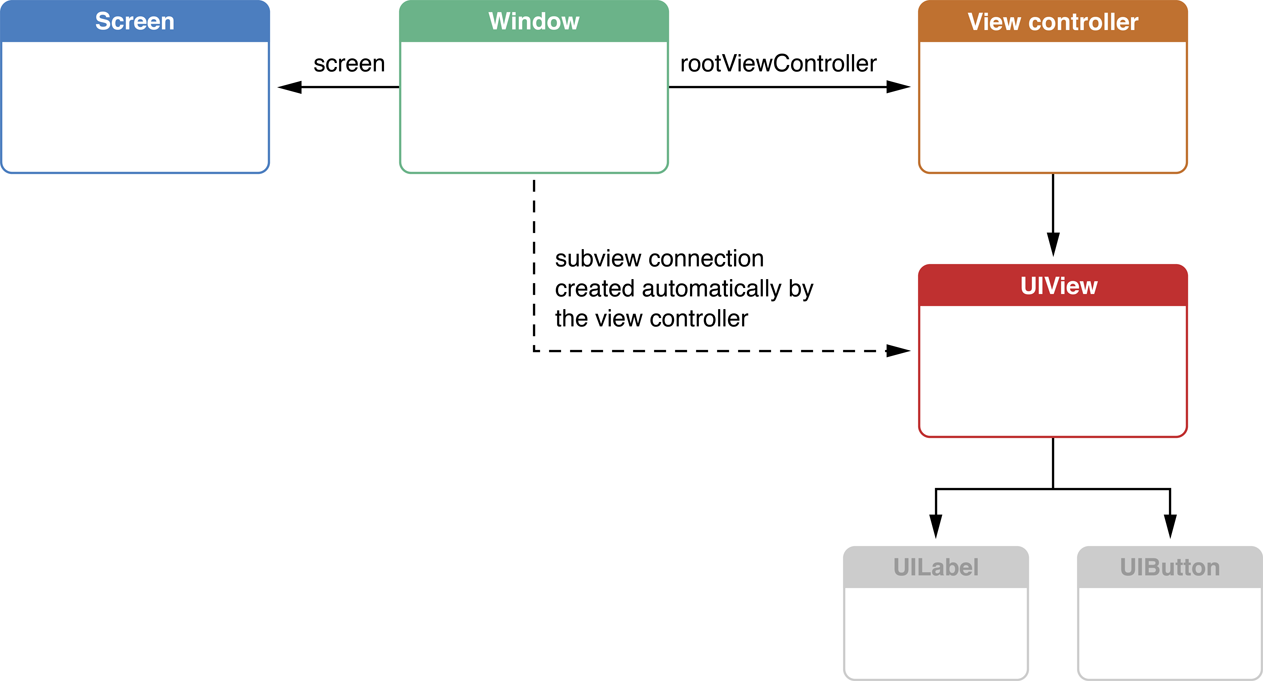
\includegraphics[totalheight=0.35\textheight]{figuras/apple_window_view_controller_screen.png}
  \caption{Esquema relacionando os elementos da UI}
  \label{fig:a}
\end{figure}

\bigskip

\subsection{UIView x UIViewController}

\paragraph{}Um objeto do tipo \texttt{\textbf{UIView}}, ou apenas \emph{View}, é onde colocamos de fato os elementos visuais. Ela representa uma determinada área onde pode conter objetos como \texttt{\textbf{UIButton}}, \texttt{\textbf{UILabel}} e \texttt{\textbf{UITextField}}, além de outras \emph{Views} inseridas, formando uma hierarquia de objetos que vão se orientar diretamente pelo posicionamento e comportamento da \texttt{\textbf{UIView}} maior.
\paragraph{}A grande ideia a ser entendida e que diferencia uma \emph{View} de uma \emph{View Controller} é que um objeto de \texttt{\textbf{UIView}} contém estritamente elementros gráficos, sem nenhuma lógica do comportamento. Um objeto de \texttt{\textbf{UIView}} não entende e não deve entender as consequências de suas ações. Um UIButton, por exemplo, sabe como agir quando é clicado mas não sabe qual tipo de ação ou mensagem foi gerada e nem pra onde ela foi a partir do seu clique.
\paragraph{}Deixando algumas coisas claras, uma tela pode conter uma só \emph{View} tomando todo o espaço ou várias \emph{Views} se divindido, sendo elas totalmente independentes ou aninhadas. Além disso, você pode criar novas classes herdando de \texttt{\textbf{UIView}} para serem estanciadas dentro de uma \texttt{\textbf{UIViewController}}.\\

\paragraph{}Uma \emph{View Controller} é o que gerencia a lógica e comportamento de um conjunto específico de uma ou mais \emph{Views}, e é responsável por carregar e interagir com as \emph{Views} na hora correta e da forma correta. Um \texttt{\textbf{UIButton}} clicado envia um sinal para a \emph{View Controller}, que tem o papel de entender qual deve ser a resposta para esse evento, que pode ser algo como envio de dados, interação com as \emph{Views}, ou criação de animações.
\paragraph{}Uma \emph{View Controller} é criada com uma única \emph{View} atrelada. É possível então adicionar mais \emph{Views} dentro da \emph{View} principal ou em conjunto com ela.
\paragraph{}Sabendo que é possível criar uma classe para uma \emph{View} genérica, sem possuir uma \emph{View Controller} atrelada, como sabemos se criamos uma classe herdando de\texttt{\textbf{UIView}} ou de \texttt{\textbf{UIViewController}}? Essa pergunta pode causar confusão no início, mas fica mais claro após entender exatamente o papel de cada uma.
\paragraph{}Primeiramente seguimos a regra de que para cada tela completa criamos uma \emph{View Controller} para gerenciá-la, e nessa classe podemos inserir todos os elementos da tela. Porém há os casos em que a ideia é criar uma \emph{View} genérica a ser inserida no contexto de uma tela completa, \emph{View} essa que pode ser desde uma célula customizada para uma tabela até uma tabela completa, aí então devemos pensar se essa mesma \emph{View} terá algum comportamento ou se será unicamente visual. No caso de uma célula customizada, por exemplo, ela será apenas visual e assim deve ser uma simples classe de \texttt{\textbf{UIView}}; já no caso de uma tabela completa, ela vai precisar de um grande conjunto de lógica para o seu comportamento, portanto precisará de uma \emph{View Controller} própria, que no caso de tabelas tem uma classe especial chamada \texttt{\textbf{UITableViewController}}.

\bigskip

\subsection{Navegação entre telas}

\bigskip

\begin{figure}[h]
  \centering
  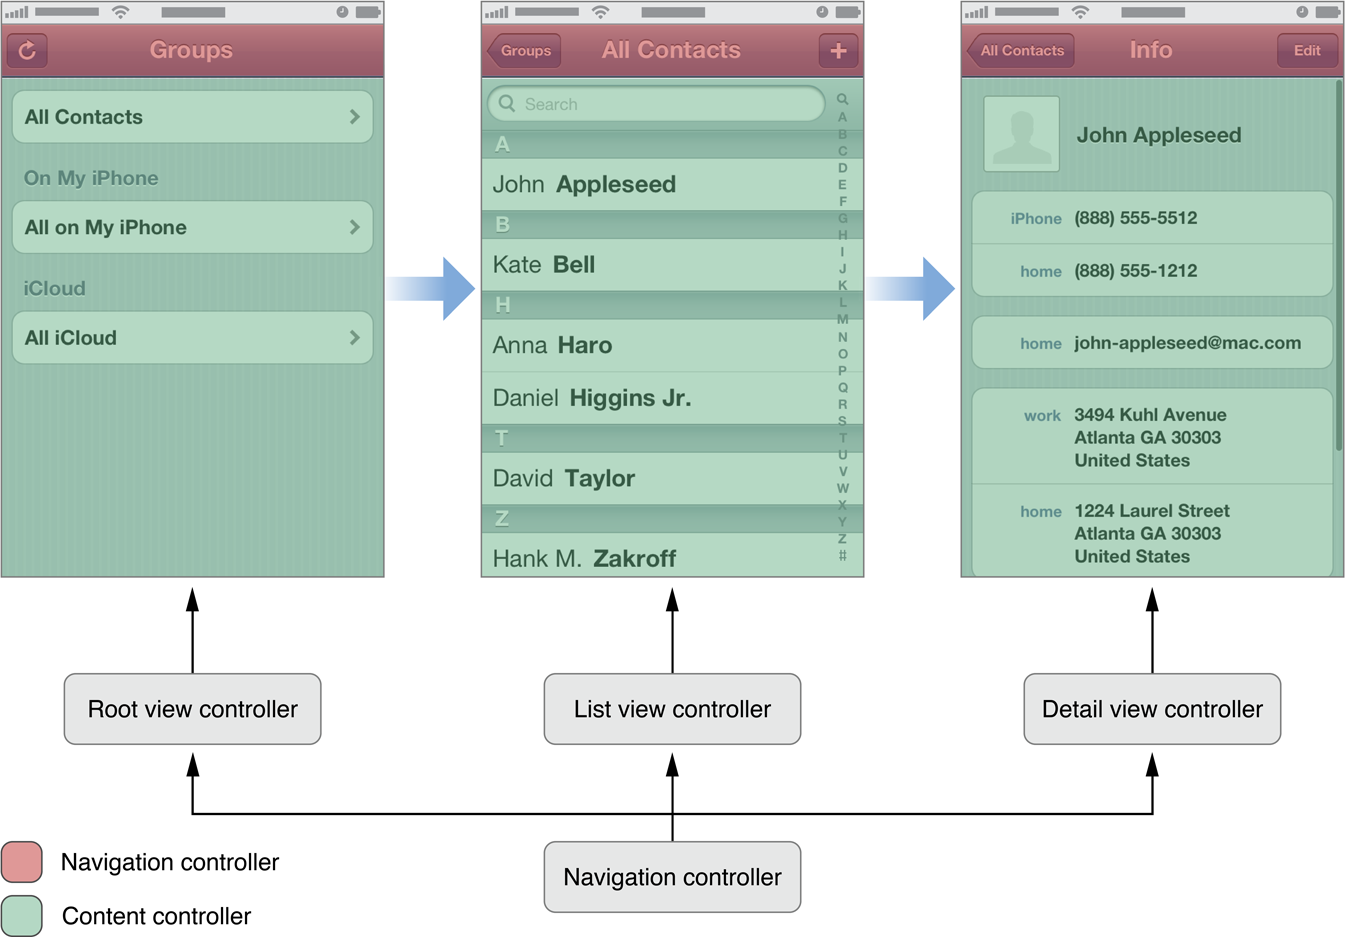
\includegraphics[totalheight=0.35\textheight]{figuras/apple_navigation_interface.png}
  \caption{Esquema do funcionamento do Navigation Controller}
  \label{fig:a}
\end{figure}

\bigskip

\paragraph{}Conforme vamos criando novas telas, precisamos de um modo de chamá-las e de retornar delas para a tela anterior. O iOS permite mais de um tipo de gerenciamento de navegação das telas, mas em quase 100\% dos casos faremos uso do \emph{Navigation Controller}.
\paragraph{}O \emph{Navigation Controller} funciona como uma pilha de \emph{View Controllers} que tem início sempre na já citada \texttt{\textbf{RootNavigationController}}, que será a tela inicial do aplicativo. Definimos uma única vez pelo código qual será nossa \texttt{\textbf{RootNavigationController}}, após isso trabalharemos apenas com métodos de \emph{push} e \emph{pop} para carregar e descarregar as telas. Graficamente, o \emph{Navigation Controller} é a barra superior (que também pode ser inferior) nas telas dos aplicativos e que contém um botão de retorno e outros botões auxiliares.
\paragraph{}Há um outro tipo de navegação complementar chamado \emph{Tab Bar Controller}, que nada mais é que uma nova tela, que pode inclusive estar contida na pilha do \emph{Navigation Controller}, e que traz duas ou mais telas divididas por abas.

\bigskip

\begin{figure}[h]
  \centering
  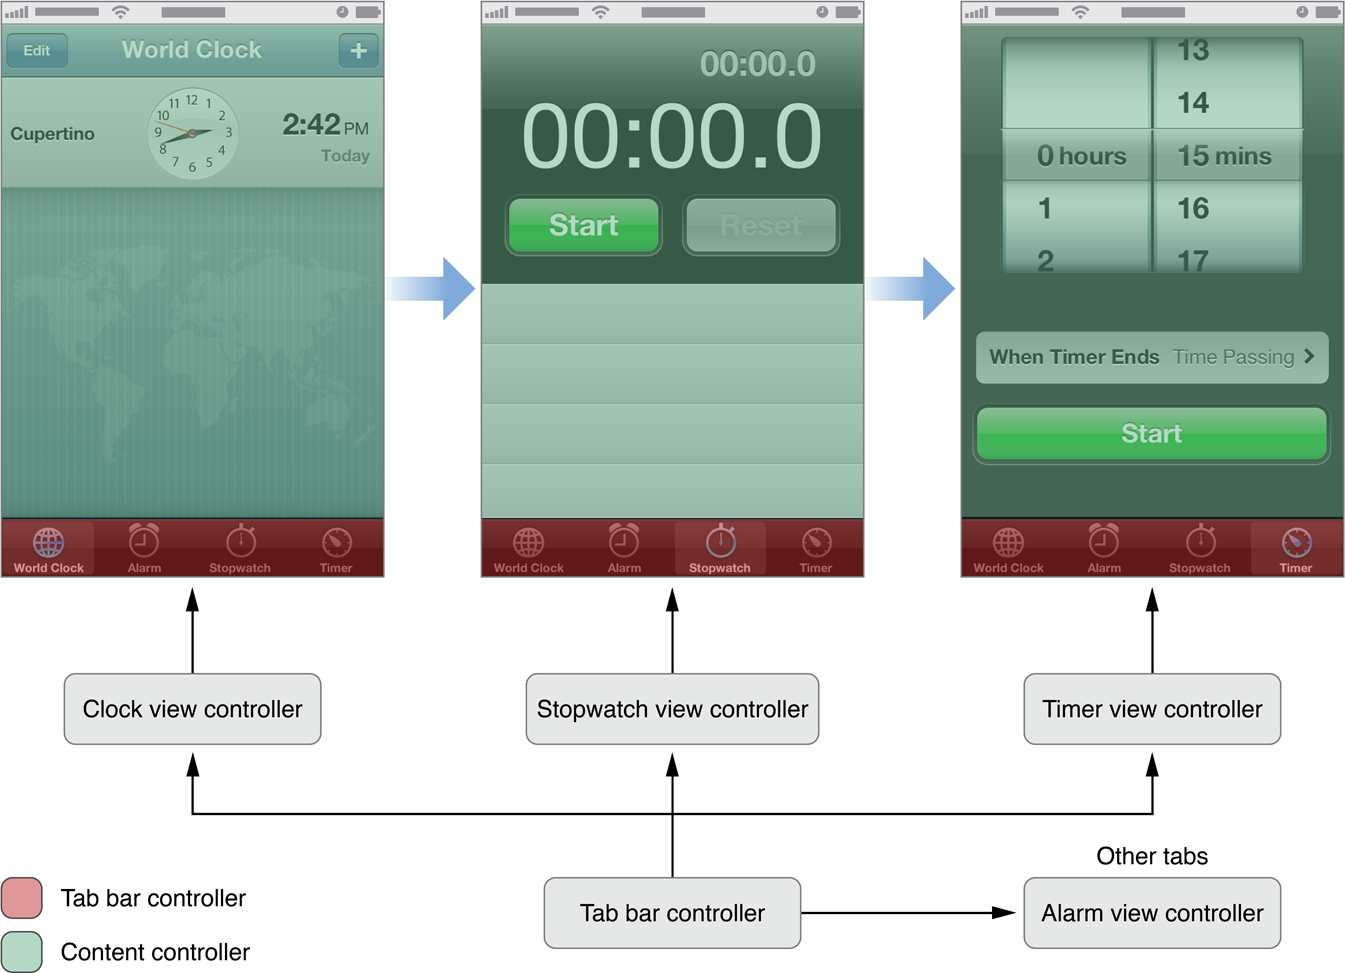
\includegraphics[totalheight=0.4\textheight]{figuras/apple_tabbar_interface.png}
  \caption{Esquema do funcionamento do Tab Bar Controller}
  \label{fig:a}
\end{figure}

\bigskip
\bigskip


\section{Interface Builder}

\paragraph{}Para nos auxiliar na construção das telas, utilizeremos o Interface Builder do XCode. Na criação de uma nova \emph{View Controller}, é criado um arquivo *.xib atrelado a essa classe, que ligará automaticamente os objetos criados na interface ao código da classe.
\paragraph{}O Interface Builder é uma ferramente muito poderosa e o utilizaremos principalmente para definir o posicionamento dos objetos, como as \emph{Views} e seus componentes, e para fazer a ligação dos \texttt{\textbf{outlets}} e \texttt{\textbf{actions}} ao código.
\paragraph{}E lembrando que sempre podemos determinar o layout e a criação dos objetos diretamente no código, sendo o Interface Builder apenas um facilitador. Em diversos casos lidar com o código acaba sendo até mais prático.

\bigskip

\subsection{Outlets e Actions}

\paragraph{}\texttt{\textbf{Outlets}} representam uma ligação entre um objeto criado na interface pelo Interface Builder, como um botão ou um texto, e uma instância criada no código. Funciona como um ponteiro de um objeto do código para a sua representação gráfica, e assim podemos nos referenciar a esse elemento no código do \emph{View Controller} para definirmos seu comportamento e possíveis mudanças nas suas características.
\paragraph{}Já uma \texttt{\textbf{action}} representa uma mensagem enviada por um objeto na interface. A \emph{action} define o tipo de toque que aciona a mensagem e cria o método que será chamado e conterá o código do programador para definir o comportamento desejado.

\bigskip
\bigskip


\section{Seu primeiro aplicativo}

\paragraph{}Agora vamos enfim colocar a mão na massa e colocar em ordem tudo que foi falado até agora.
\paragraph{}Abra o XCode e escolha a opção de criar um novo projeto. Na nova janela aberta, escolha a opção \emph{Single View Application} e siga em frente.

\begin{figure}[h]
  \centering
  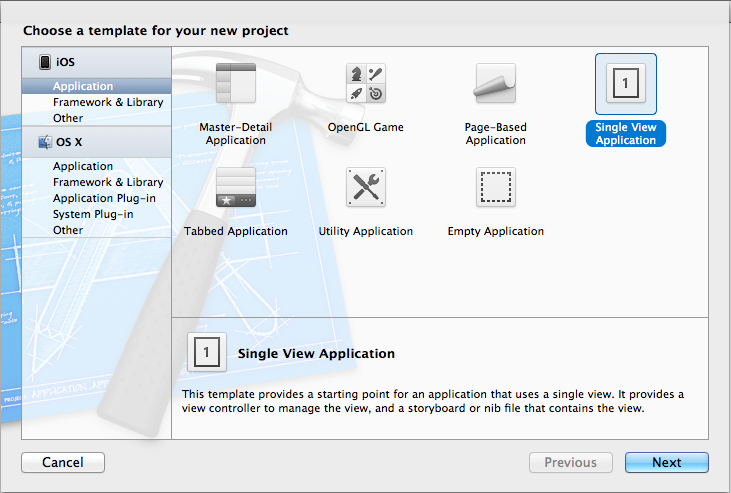
\includegraphics[totalheight=0.3\textheight]{figuras/1/novo_projeto1.png}
  \caption{Criação do novo projeto}
  \label{fig:a}
\end{figure}

\bigskip

\paragraph{}Na próxima tela você pode escolher os detalhes do aplicativo. Tenha certeza que a opção \emph{Use Automatic Reference Counting} está marcada.

\begin{figure}[h]
  \centering
  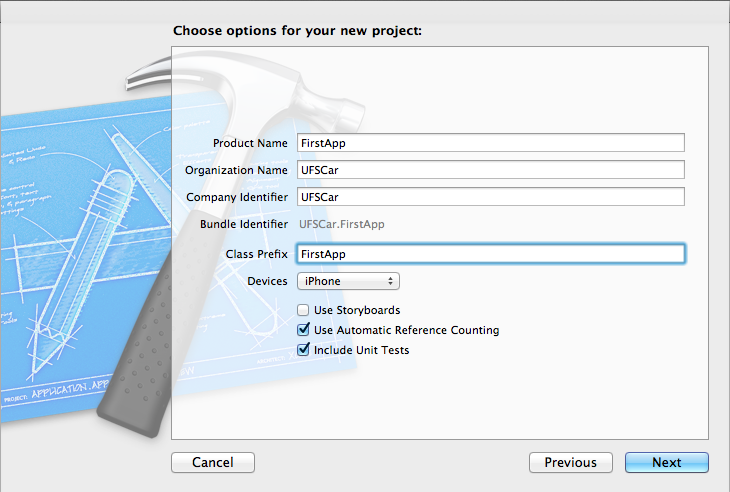
\includegraphics[totalheight=0.3\textheight]{figuras/1/novo_projeto2.png}
  \caption{Criação do novo projeto}
  \label{fig:a}
\end{figure}

\bigskip

\paragraph{}Conclua a criação do projeto, com a opção \emph{Create an .xib file} marcada. Podemos agora visualizar a classe mãe do projeto, que será responsável pela tela inicial do aplicativo.
\paragraph{}Para visualizar melhor os arquivos do projeto, use os ícones acima de Editor no canto superior direito para escolher a forma da exibição do código.

\begin{figure}[h]
  \centering
  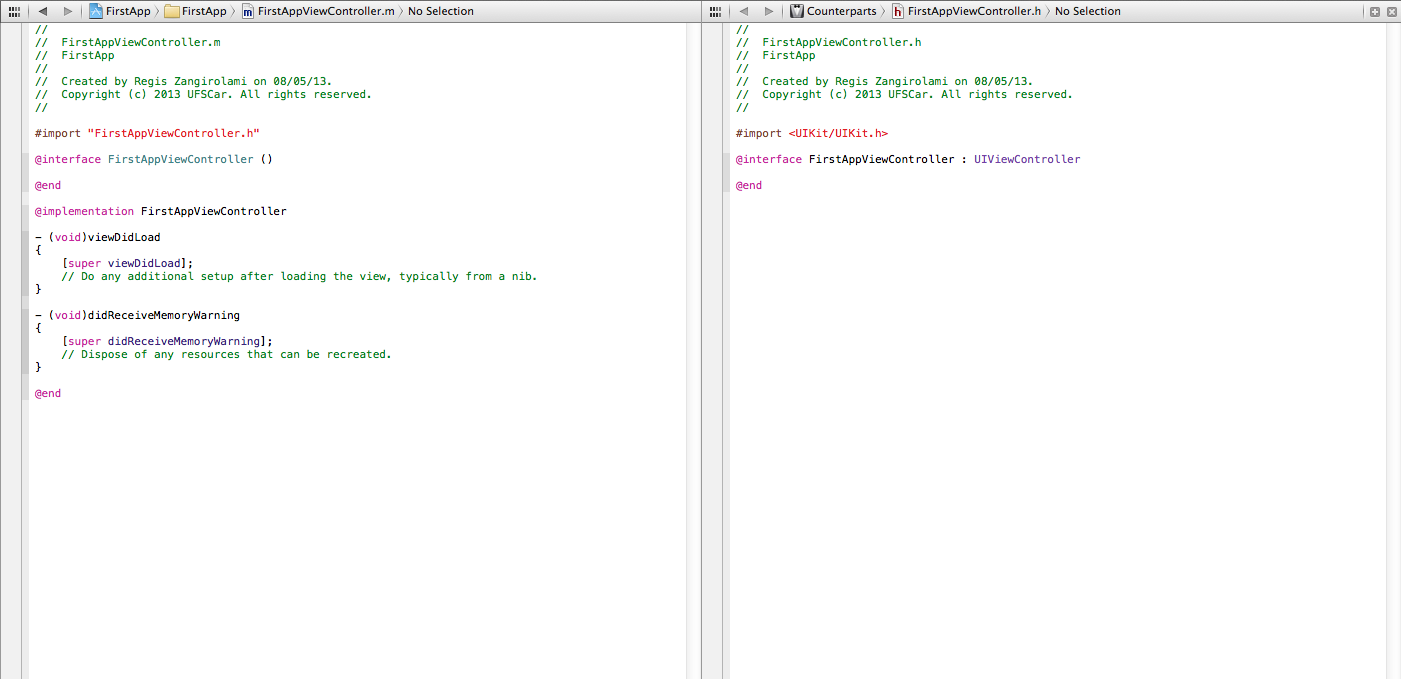
\includegraphics[totalheight=0.3\textheight]{figuras/1/codigo_classe_mh.png}
  \caption{Tela dividida com os dois arquivos de código da classe}
  \label{fig:a}
\end{figure}

\bigskip

\subsection{Primeira tela}

\paragraph{}No lado esquerdo está o navegador dos arquivos do projeto. Selecione o arquivo .xib da classe para abrir o Interface Builder.

\begin{figure}[h]
  \centering
  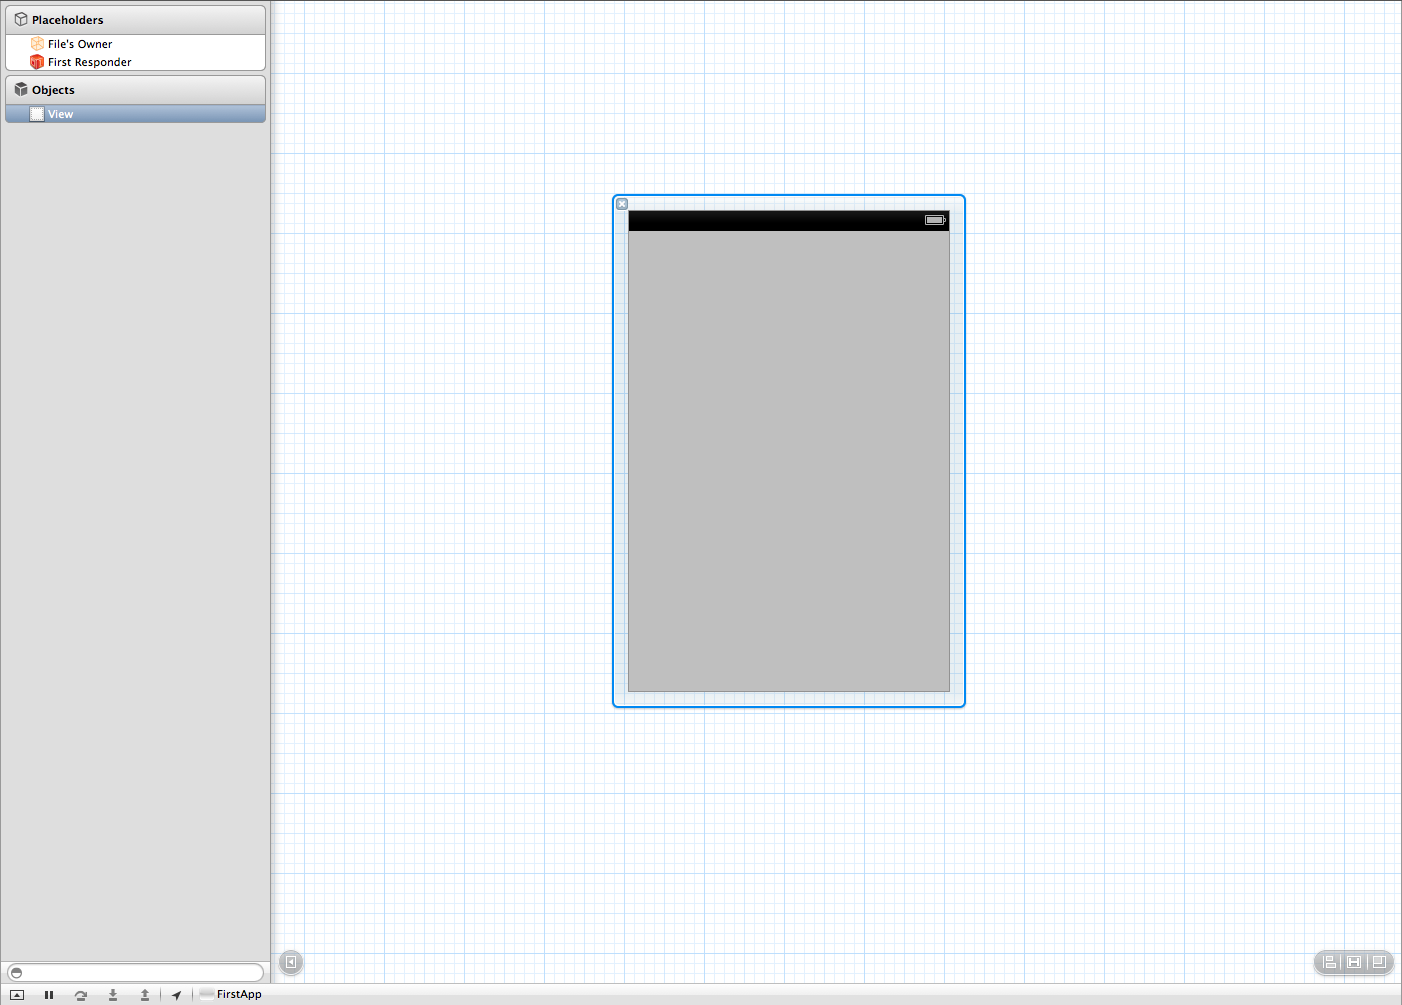
\includegraphics[totalheight=0.25\textheight]{figuras/1/xib.png}
  \caption{Arquivo xib da primeira tela}
  \label{fig:a}
\end{figure}

\bigskip

\paragraph{}No canto superior direito, entre os acima de View, clique no ícone da direita  para abrir a seção de opções do Interface Builder. Nessa parte poderemos ver e editar as características de qualquer objeto selecionado da tela, desde um botão a uma View, e alternar as opções entre as abas.

\begin{figure}[h]
  \centering
  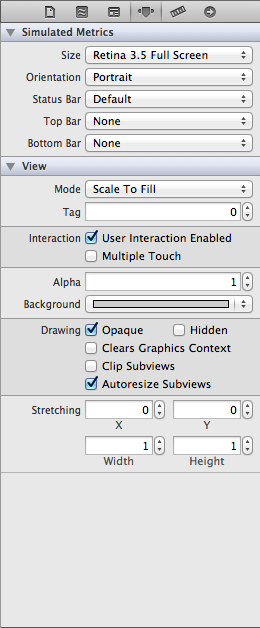
\includegraphics[totalheight=0.35\textheight]{figuras/1/xib_opcoes.png}
  \caption{Barra lateral de opções do Interface Builder}
  \label{fig:a}
\end{figure}

\bigskip

\paragraph{}Podemos selecionar e arrastar à tela qualquer objeto. Esses objetos estão presentes na seção de objetos no canto inferior esquerdo.

\begin{figure}[h]
  \centering
  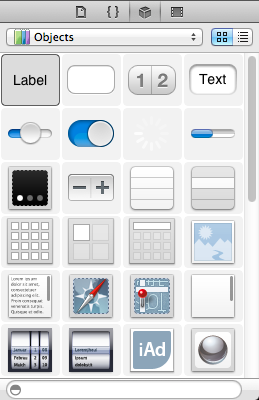
\includegraphics[totalheight=0.25\textheight]{figuras/1/xib_objetos.png}
  \caption{Objetos disponíveis no Interface Builder}
  \label{fig:a}
\end{figure}

\bigskip

\paragraph{}Vamos inicialmente adicionar um \texttt{\textbf{UILabel}} e um \texttt{\textbf{UIButton}} com textos de exemplo à tela.

\begin{figure}[h]
  \centering
  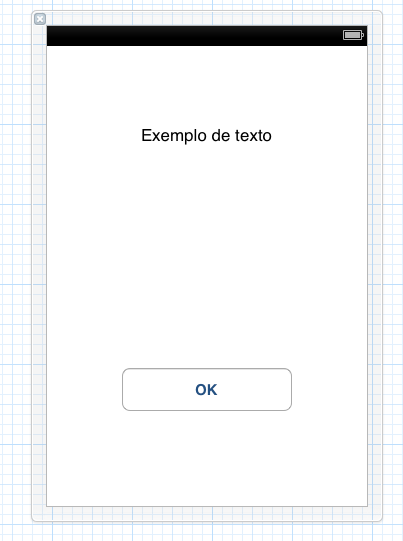
\includegraphics[totalheight=0.4\textheight]{figuras/1/xib_tela1.png}
  \caption{Interface com os primeiros objetos criados}
  \label{fig:a}
\end{figure}

\paragraph{}Com os objetos adicionados, devemos ligá-los ao código. Para isso, basta selecionar o objeto e arratá-lo ao código da classe enquanto segura a tecla Ctrl.
\paragraph{}No pop-up é possível escolher se é um \texttt{\textbf{•}f{outlet}} ou uma \texttt{\textbf{action}}, mas por enquanto criaremos só os \emph{outlets}. Escolha um nome apropriado ao objeto, que o diferencie mas também deixe claro o seu tipo para facilitar a leitura do código.

\begin{figure}[h]
  \centering
  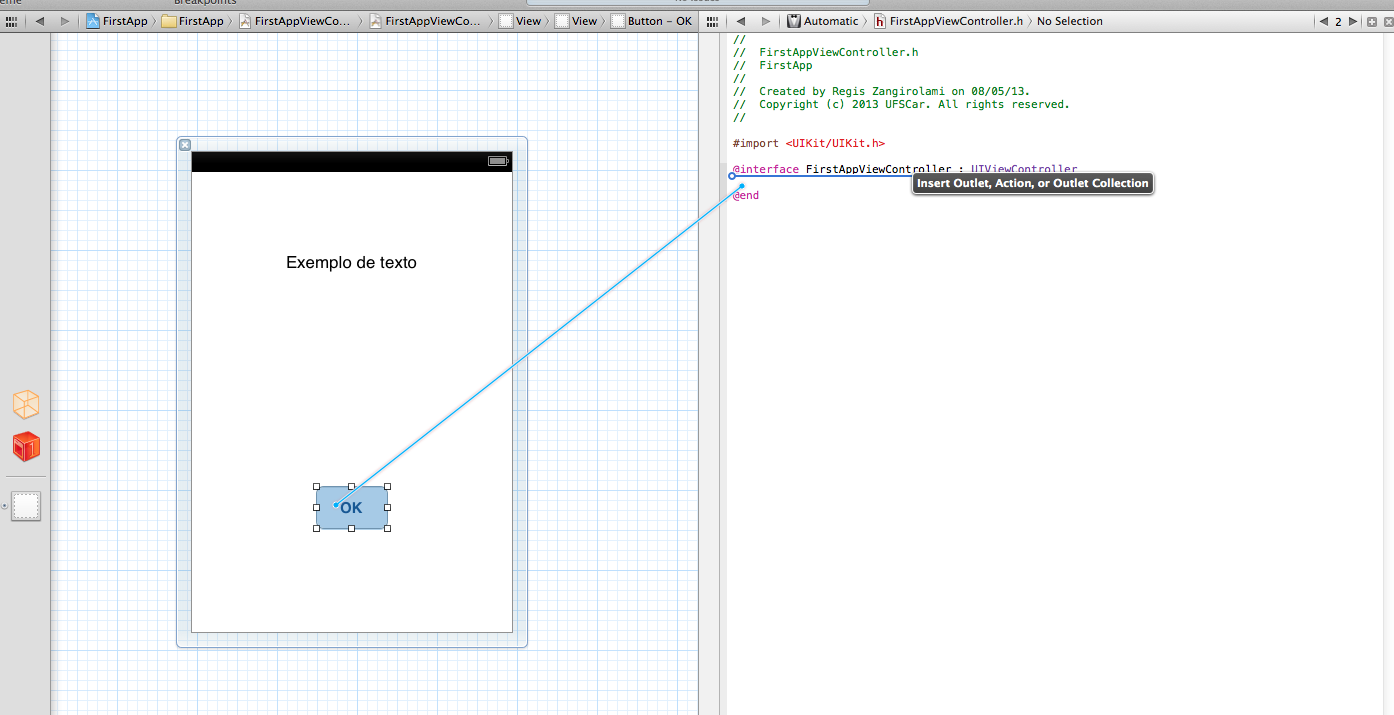
\includegraphics[totalheight=0.25\textheight]{figuras/1/link_outlet_button.png}
  \caption{Outlets: ligação dos objetos com o código}
  \label{fig:a}
\end{figure}

\paragraph{}Agora precisamos definir o funcionamento do Navigation Controller. Abra o arquivo FirstAppAppDelegate.h e adicione a seguinte property:

\begin{listing}
\begin{minted}[linenos=true,frame=lines,framesep=2mm,tabsize=2,numbersep=5pt]{objective-c}
@property (strong, nonatomic) UINavigationController *navController;
\end{minted}
\end{listing}

\paragraph{}E no arquivo FirstAppAppDelegate.m, deixaremos o primeiro método desse jeito:

\begin{listing}
\begin{minted}[linenos=true,frame=lines,framesep=2mm,tabsize=2,numbersep=5pt]{objective-c}
- (BOOL)application:(UIApplication *)application
didFinishLaunchingWithOptions:(NSDictionary *)launchOptions
{
    self.window = [[UIWindow alloc] initWithFrame:
                  [[UIScreen mainScreen] bounds]];
    
    self.viewController = [[FirstAppViewController alloc]
                initWithNibName:@"FirstAppViewController" bundle:nil];
    self.navController = [[UINavigationController alloc]
                initWithRootViewController:self.viewController];
   
    self.window.rootViewController = self.navController;
    [self.window makeKeyAndVisible];
    
    return YES;
}
\end{minted}
\end{listing}

\paragraph{}Nesse arquivo é inicializado a \texttt{\textbf{UIWindow}} e a \texttt{\textbf{UIScreen}}, já citadas aqui. Como foi dito, a \texttt{\textbf{UIWindow}} é a reponsável por chamar a primeira tela do aplicativo. Nesse código é criado a Navigation Controller que utilizaremos para navegar entre as telas do aplicativo, e definimos qual será a primeira tela, chamada \texttt{\textbf{RootNavigationController}}.
\paragraph{}E pronto, com a Navigation Controller criadao não mexeremos mais nesse arquivo.\\

\paragraph{}Voltando à classe da primeira tela, podemos agora criar um título para a tela, que aparecerá na barra de navegação. No método \texttt{\textbf{viewDidLoad}} adicione a linha:

\begin{listing}
\begin{minted}[linenos=true,frame=lines,framesep=2mm,tabsize=2,numbersep=5pt]{objective-c}
self.navigationItem.title = @"Tela 1";
\end{minted}
\end{listing}

\paragraph{}O método \texttt{\textbf{viewDidLoad}} é onde colocaremos tudo que será setado no carregamento da tela, é o método de inicalização. Há um grande número de métodos do \texttt{\textbf{UIViewController}} que podemos sobreescrever de acordo com a nossa necessidade. Eles têm a função de controlar o comportamento da tela durante toda a existência da tela, desde sua inicialização até finalização, podendo prever respostas a ações do usuário.
\paragraph{}Agora o aplicativo ainda está extremamente cru, mas já podemos executá-lo no \emph{iOS Simulator} para ver sua primeira aparência. Basta apertar o botão Play no canto superior esquerdo.

\begin{figure}[h]
  \centering
  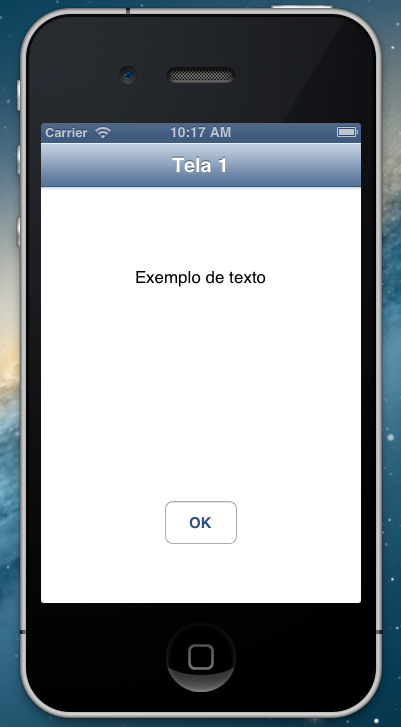
\includegraphics[totalheight=0.4\textheight]{figuras/1/simulador1_tela1.png}
  \caption{Aplicativo executando no iOS Simulator}
  \label{fig:a}
\end{figure}

\bigskip

\paragraph{}Podemos agora começar a brincar com o código. Vamos criar uma \texttt{\textbf{action}} bem simples para testarmos o comportamento do aplicativo com o simulador. Para isso basta arrastar segurando Ctrl do botão para o código e escolher a opção \texttt{\textbf{action}}, e criar um nome para ela. A intenção da nossa primeira \texttt{\textbf{action}} é que os textos do botão e do label troquem quando clicarmos no botão.
\paragraph{}Com a \texttt{\textbf{action}} criada, veja que no código de implementação da classe (arquivo *.m) já tem o esqueleto do método que será chamado, e nele colocaremos nossa lógica.

\begin{listing}
\begin{minted}[linenos=true,frame=lines,framesep=2mm,tabsize=2,numbersep=5pt]{objective-c}
- (IBAction)okTouched:(id)sender {
    
    NSString *aux = [[NSString alloc] initWithString:
                    self.exemploLabel.text];
    self.exemploLabel.text = self.okButton.currentTitle;
    [self.okButton setTitle:aux forState:UIControlStateNormal];
}
\end{minted}
\end{listing}

\paragraph{}O código funciona como um simples swap. Na linha 3 temos inicializamos uma variável local com o texto do label; na linha 4 atribuimos o texto do botão ao texto do label; e na linha 5 chamamos o método da classe \texttt{\textbf{UIButton}} responsável por setar o texto do botão, que no caso será o texto salvo na variável auxiliar.
\paragraph{}Rode o aplicativo no simulador para verificar o funcionamento do botão.\\

\bigskip

\subsection{Manipulando o Navigation Controller}

\paragraph{}Pensando agora na próxima tela, vamos preparar o terreno para a transição. Adicionamos um novo botão que servirá de chamada para a segunda tela, e criamos um \texttt{\textbf{outlet}} e uma \texttt{\textbf{action}} para ele. Colocaremos no método da \texttt{\textbf{action}} a chamada para a segunda tela, que será através de um \emph{push} da tela no Navigation Controller.

\begin{listing}
\begin{minted}[linenos=true,frame=lines,framesep=2mm,tabsize=2,numbersep=5pt]{objective-c}
- (IBAction)secondScreenTouched:(id)sender {
    
    self.secondScreen = [[SecondScreenViewController alloc]
                        initWithNibName:
                        @"SecondScreenViewController" bundle:nil];
    
    [self.navigationController pushViewController:self.secondScreen
                                         animated:YES];
}
\end{minted}
\end{listing}

\paragraph{}Para chamar uma nova tela é preciso criar uma instância da \emph{View Controller} a ser chamada, no caso da SecondScreenViewController (que ainda não criamos), para então jogá-la na pilha com o método de \emph{push}, que recebe como parâmetro a instância criada.
\paragraph{}A nossa tela deve estar parecida com essa:

\begin{figure}[h]
  \centering
  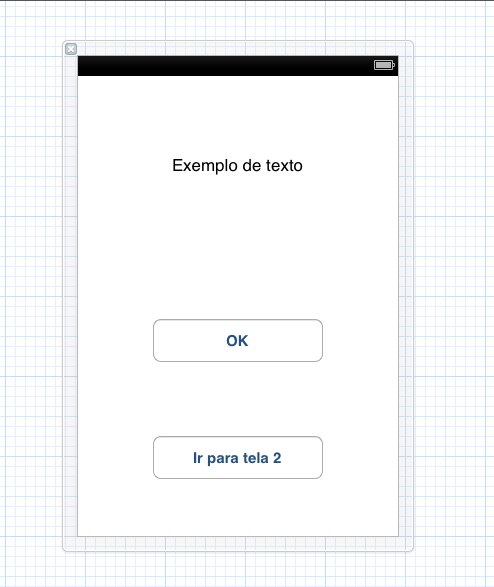
\includegraphics[totalheight=0.3\textheight]{figuras/1/simulador3_tela1.png}
  \caption{Primeira tela com o botão de chamada da segunda tela}
  \label{fig:a}
\end{figure}

\paragraph{}Agora podemos criar a segunda tela. Criamos um novo arquivo em New, definimos a herança da classe, que no caso de uma tela é uma \texttt{\textbf{UIViewController}}, e seu nome, que no exemplo será SecondScreenViewController. É importante que o nome da classe seja exatamente como está no código da criação.
\paragraph{}Nessa segunda tela vamos colocar uma \texttt{\textbf{UIImage}}, arrastando da mesma forma que os outros objetos, e por enquanto mais um botão que fará a chamada da terceira tela.

\begin{figure}[h]
  \centering
  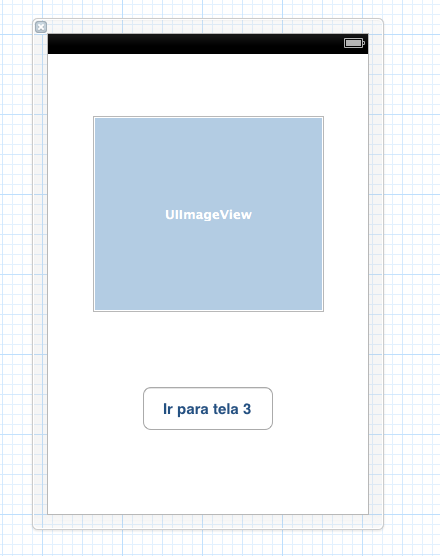
\includegraphics[totalheight=0.25\textheight]{figuras/2/xib_tela2.png}
  \caption{Tela 2 com UIImage sem imagem}
  \label{fig:a}
\end{figure}

\bigskip

\paragraph{}Devemos agora definir uma imagem para a \texttt{\textbf{UIImage}}, mas antes é preciso adicionar a imagem que queremos na pasta Supporting Files do projeto. Para isso, basta clicar com o botão direito na pasta e adicionar os arquivos em Add Files to "First App".

\begin{figure}[h]
  \centering
  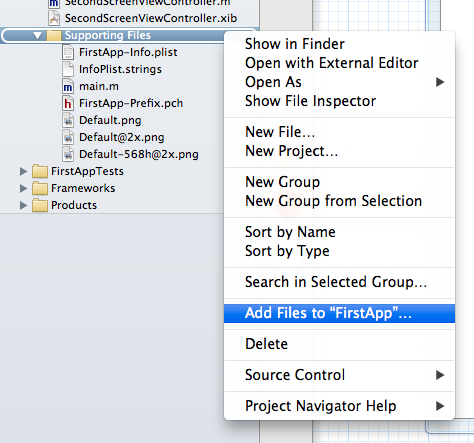
\includegraphics[totalheight=0.3\textheight]{figuras/2/add_files.png}
  \caption{Adicionando arquivos ao projeto}
  \label{fig:a}
\end{figure}

\paragraph{}Adicionamos a imagem LogoDC.png contida neste tutorial. Depois de adicionada, selecionamos a \texttt{\textbf{UIImage}} e setamos o nome da imagem na barra lateral de opções.

\begin{figure}[h]
  \centering
  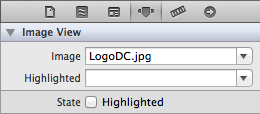
\includegraphics[totalheight=0.12\textheight]{figuras/2/image_path.png}
  \caption{Setando a imagem}
  \label{fig:a}
\end{figure}

\begin{figure}[!h]
  \centering
  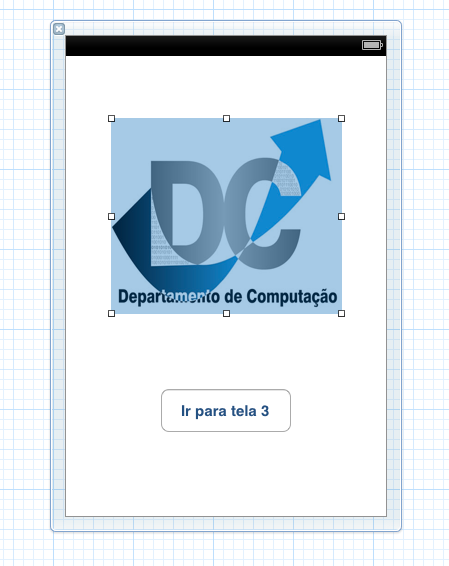
\includegraphics[totalheight=0.25\textheight]{figuras/2/xib2_tela2.png}
  \caption{Imagem aparecendo na tela}
  \label{fig:a}
\end{figure}

\paragraph{}Para dar funcionalidade ao botão, crie a terceira tela com o nome ThirdScreenViewController, seguindo o exemplo, e faça a chamada da mesma forma que foi feito na primeira tela.

\bigskip

\subsection{Trocando informação entre telas}

\paragraph{}Ao inicializarmos uma instância de uma \emph{View Controller}, podemos atribuir valores às suas Properties antes de fazer o \emph{push} da tela. Dessa forma bem simples, é possível levar informação de uma tela existente para uma tela nova, podendo exibir ou tratar esses dados convenientemente na \emph{View Controller} da próxima tela. Para exemplificar, vamos criar um campo de texto na segunda tela e exibir o seu conteúdo em um label na terceira tela.
\paragraph{}Para isso vamos precisar de um campo de texto na segunda tela, de um label na terceira tela, e de uma variável do tipo string na terceira tela, onde vamos armazenar o conteúdo do text field. Além disso, também é preciso criar a \texttt{\textbf{action}} para fazer a chamada da terceira tela pelo botão.
\paragraph{}A \texttt{\textbf{Property}} da string é criada no arquivo de header da classe da terceira tela da seguinte forma:

\begin{listing}
\begin{minted}[linenos=true,frame=lines,framesep=2mm,tabsize=2,numbersep=5pt]{objective-c}
@property (nonatomic, strong) NSString *textLabel;
\end{minted}
\end{listing}

\paragraph{}A segunda tela e suas propriedades devem estar assim:

\begin{figure}[h]
  \centering
  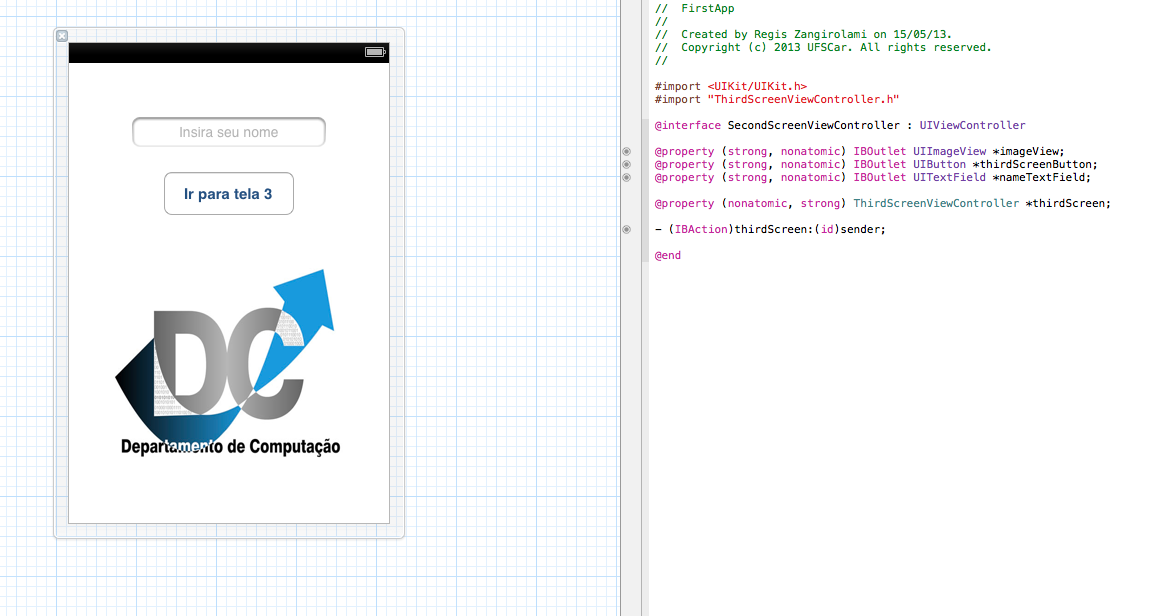
\includegraphics[totalheight=0.3\textheight]{figuras/2/xib_tela2_header.png}
  \caption{Tela 2 e seus outlets}
  \label{fig:a}
\end{figure}

\bigskip
\bigskip

\paragraph{}E o método com a chamada da terceira tela será quase do mesmo jeito, apenas com a adição da passagem da variável.

\begin{listing}
\begin{minted}[linenos=true,frame=lines,framesep=2mm,tabsize=2,numbersep=5pt]{objective-c}
- (IBAction)thirdScreen:(id)sender {
    
    self.thirdScreen = [[ThirdScreenViewController alloc]
                       initWithNibName:@"ThirdScreenViewController"
                       bundle:nil];
    
    self.thirdScreen.textLabel = self.nameTextField.text;
    
    [self.navigationController pushViewController:self.thirdScreen
                                         animated:YES];
}
\end{minted}
\end{listing}

\bigskip

\paragraph{}Além disso, precisamos tratar o conteúdo da variável na classe da terceira tela. Vamos verificar no método \texttt{\textbf{viewDidLoad}} o conteúdo da variável que recebeu o dado da segunda tela.

\begin{listing}
\begin{minted}[linenos=true,frame=lines,framesep=2mm,tabsize=2,numbersep=5pt]{objective-c}
- (void)viewDidLoad
{
    [super viewDidLoad];
    
    if (![self.textLabel isEqualToString:@""]) {
        self.nameLabel.text = self.textLabel;
    } else {
        self.nameLabel.text = @"Sem nome";
    }
    
    self.messageTextField.delegate = self;
}
\end{minted}
\end{listing}

\bigskip

\paragraph{}De uma forma bem simples, verificamos o conteúdo da string recebida e setamos o conteúdo do nosso label.
\paragraph{}Note que único problema agora será após a edição do campo de texto na segunda tela, já que o teclado sobre mas não abaixa automaticamente. Deixaremos assim por enquanto. Tente posicionar o campo de texto e o botão de forma que o teclado não os cubra, apenas para verificar o funcionamento do código. Resolveremos o problema do teclado mais a frente.
\paragraph{}Aqui uma imagem da segunda tela no simulador.\\

\bigskip
\bigskip

\begin{figure}[h]
  \centering
  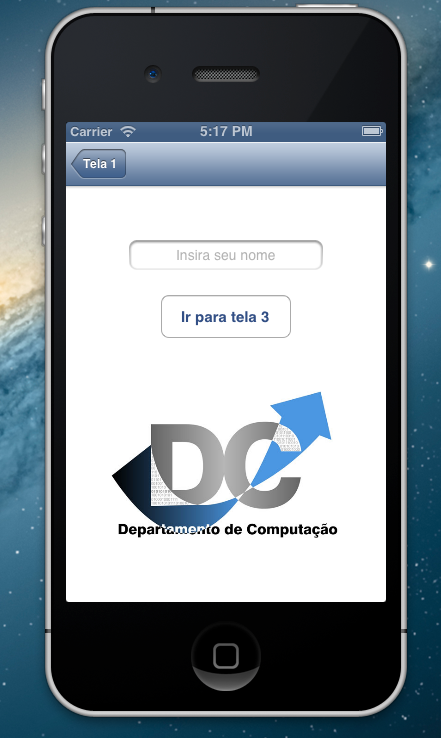
\includegraphics[totalheight=0.4\textheight]{figuras/2/simulador2_tela2.png}
  \caption{Tela 2 completa}
  \label{fig:a}
\end{figure}

\bigskip

\subsection{O uso do protocolo Delegate}

\paragraph{}O protocolo \texttt{\textbf{Delegate}} é uma das ferramentas mais importantes do Objective-C. Na execução do código de um objeto, este não tem como ter acesso código do objeto que o instanciou. Com o uso do \texttt{\textbf{Delegate}} um objeto pode enviar dados para um segundo objeto que enxerga o primeiro mas não pode ser enxergado por ele. Assim é possível determinar que a partir de um evento ou uma condição, será enviada uma mensagem, que pode ser uma notificação ou um dado, a partir de um método \texttt{\textbf{Delegate}} que vai saber como e onde encontrar o destino dessa mensagem.
\paragraph{}Veremos dois exemplos de uso do \texttt{\textbf{Delegate}} no nosso aplicativo. No primeiro usaremos um método já pronto, que será responsável por enviar o aviso para o teclado de que o campo de texto já terminou de ser usado e ele agora deve desaparecer. No segundo vamos implementar um método para enviar uma string da terceira tela para a tela que a chamou, no nosso caso a segunda tela.

\paragraph{}Utilizar o \texttt{\textbf{Delegate}} já implementado do \texttt{\textbf{UITextField}} será bem simples. Faremos uma referência no header das classes em que utilizamos o teclado em um \texttt{\textbf{UITextField}}, no caso a segunda e terceira tela. Fazemos dessa forma:

\begin{listing}
\begin{minted}[linenos=true,frame=lines,framesep=2mm,tabsize=2,numbersep=5pt]{objective-c}
@interface SecondScreenViewController :
           UIViewController <UITextFieldDelegate>
\end{minted}
\end{listing}

\paragraph{}A referência a um \texttt{\textbf{Delegate}} vem sempre entre < e > na declaração da classe, separando por vírgula dentro da chave se houver mais de um. Após isso, precisamos apenas atribuir o \texttt{\textbf{Delegate}} à classe no \texttt{\textbf{viewDidLoad}}.

\begin{listing}
\begin{minted}[linenos=true,frame=lines,framesep=2mm,tabsize=2,numbersep=5pt]{objective-c}
self.nameTextField.delegate = self;
\end{minted}
\end{listing}

\paragraph{}Pronto, agora é possível que o objeto \texttt{\textbf{UITextField}}, que foi instanciado na classe da tela e consequentemente não enxerga os elementos dessa classe, como o teclado, envie informações à mesma. No caso, queremos que o teclado seja dispensado no momento que terminarmos de editar o campo de texto, e quando isso ocorre há um método a ser chamado. Vamos implementar este método com a lógica que queremos no arquivo de implementação da classe.

\begin{listing}
\begin{minted}[linenos=true,frame=lines,framesep=2mm,tabsize=2,numbersep=5pt]{objective-c}
- (BOOL)textFieldShouldReturn:(UITextField *)textField {
    
    if (textField == self.nameTextField) {
        [textField resignFirstResponder];
    }
    
    return YES;
}
\end{minted}
\end{listing}

\paragraph{}Este código verifica se o objeto \texttt{\textbf{UITextField}} que chamou o método é o mesmo objeto instanciado na classe, no caso o \texttt{\textbf{nameTextField}}. Assim, quando há mais de um \texttt{\textbf{UITextField}}, podemos definir comportamentos diferentes para cada um apenas fazendo essa verificação.
\paragraph{}Execute o projeto e faça o teste, agora o teclado deve sumir quando o campo de texto não está selecionado.

\paragraph{}Agora vamos implementar um novo \texttt{\textbf{Delegate}} do zero para determinar o envio de informações de uma tela para a tela que a chamou. Vamos definir o \texttt{\textbf{Delegate}} na classe da terceira tela, e usar o método na segunda. Criamos um \texttt{\textbf{Protocol}} no header da classe, e dentro inserimos os métodos do \texttt{\textbf{Delegate}}, que no caso será apenas um, que terá a função de enviar como parâmetro o conteúdo de um campo de texto da terceira tela. Ficará assim:

\begin{listing}
\begin{minted}[linenos=true,frame=lines,framesep=2mm,tabsize=2,numbersep=5pt]{objective-c}
@protocol MessageDelegate <NSObject>

-(void)sendMessageFromTextField:(NSString*)message;

@end
\end{minted}
\end{listing}

\paragraph{}Então criamos uma propriedade no header para o \texttt{\textbf{Delegate}}.

\bigskip

\begin{listing}
\begin{minted}[linenos=true,frame=lines,framesep=2mm,tabsize=2,numbersep=5pt]{objective-c}
@property (assign, nonatomic) id <MessageDelegate> delegate;
\end{minted}
\end{listing}

\paragraph{}Definimos o \texttt{\textbf{Delegate}} e seu método, agora basta definir onde será a chamada do método. Criaremos um botão na terceira tela, e ligado a ela uma \emph{action} chamada \texttt{\textbf{sendMessage}}, e nesta \emph{action} ficará a chamada para o método do delegate.

\begin{listing}
\begin{minted}[linenos=true,frame=lines,framesep=2mm,tabsize=2,numbersep=5pt]{objective-c}
- (IBAction)sendMessage:(id)sender {
    
    [self.delegate sendMessageFromTextField:self.messageTextField.text];
}
\end{minted}
\end{listing}

\begin{figure}[h]
  \centering
  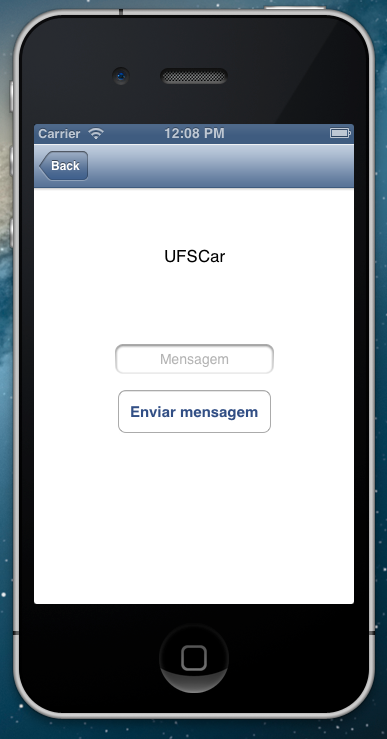
\includegraphics[totalheight=0.4\textheight]{figuras/3/simulador3_tela3.png}
  \caption{Tela 3 com o botão para enviar mensagem}
  \label{fig:a}
\end{figure}

\paragraph{}Isso determina que ao apertarmos o botão criado o método do \texttt{\textbf{Delegate}} que criamos será chamado recebendo o conteúdo do campo como parâmetro. Para receber esse conteúdo na segunda tela, faremos como no caso do teclado, implementando o método criado no \texttt{\textbf{Delegate}} com o comportamento que for desejado.

\paragraph{}Na segunda tela, faremos o mesmo processo que fizemos com o \texttt{\textbf{Delegate}} do \texttt{\textbf{UITextField}}. Adicionamos a referência ao nosso \texttt{\textbf{Delegate}} ao header.\\

\begin{listing}
\begin{minted}[linenos=true,frame=lines,framesep=2mm,tabsize=2,numbersep=5pt]{objective-c}
@interface SecondScreenViewController :
           UIViewController <UITextFieldDelegate, MessageDelegate>
\end{minted}
\end{listing}

\paragraph{}No método em que é chamada a terceira tela, atribuímos o nosso \texttt{\textbf{Delegate}} à classe da segunda tela, logo após a instanciação.

\begin{listing}
\begin{minted}[linenos=true,frame=lines,framesep=2mm,tabsize=2,numbersep=5pt]{objective-c}
- (IBAction)thirdScreen:(id)sender {
    
    self.thirdScreen = [[ThirdScreenViewController alloc] initWithNibName:@"ThirdScreenViewController" bundle:nil];
    
    self.thirdScreen.textLabel = self.nameTextField.text;
    
    self.thirdScreen.delegate = self;
    
    [self.navigationController pushViewController:self.thirdScreen animated:YES];
}
\end{minted}
\end{listing}

\paragraph{}Tudo pronto, agora basta implementar o método. Nossa intenção é que a segunda tela retorne exibindo o texto recebido da terceira tela no campo de texto, ou seja, precisamos dar um pop na terceira tela e atribuir o texto recebido por parâmetro ao \texttt{\textbf{nameTextField}}. Deve ficar assim:

\begin{listing}
\begin{minted}[linenos=true,frame=lines,framesep=2mm,tabsize=2,numbersep=5pt]{objective-c}
-(void)sendMessageFromTextField:(NSString *)message {
    
    [self.navigationController popToViewController:self animated:YES];
    
    self.nameTextField.text = message;
}
\end{minted}
\end{listing}

\bigskip


\section{Manipulando tabelas}

\paragraph{}Entre os tipos de \emph{Views} mais utilizadas no iOS, temos as tabelas. Qualquer tela exibindo informações bem divididas como playlist de músicas, lista contatos, ou informações estruturadas em linhas, é do tipo \texttt{\textbf{UITableView}} se for uma \emph{View}, ou \texttt{\textbf{UITableViewController}} se for uma controladora. Como já explicado, se for preciso apenas exibir informações estáticas sem interação com o usuário, criamos uma classe herdando de \texttt{\textbf{UITableView}}, porém na maioria dos casos vamos precisar de tabelas com dados dinâmicos e possibilidade de interação por toque, então criamos um classe herdando de \texttt{\textbf{UITableViewController}}.
\paragraph{}A classe \texttt{\textbf{UITableViewController}} possui diversos métodos para gerenciar o comportamento de uma tabela. Desde o básico para defininção do número de seções, linhas por seções e o conteúdo de cada linha, até o ajuste das ações para tipos diferentes de toque, como um toque único ou um \emph{slide} na linha para obter novas opções.
\paragraph{}Vamos implementar um exemplo simples de uma lista de contatos, exibindo-os em ordem alfabética a partir de um pré-determinado \emph{array} de objetos do tipo \texttt{\textbf{Contato}}, que será a classe modelo que criaremos para contatos com informações como nome completo e número.\\

\begin{figure}[h]
  \centering
  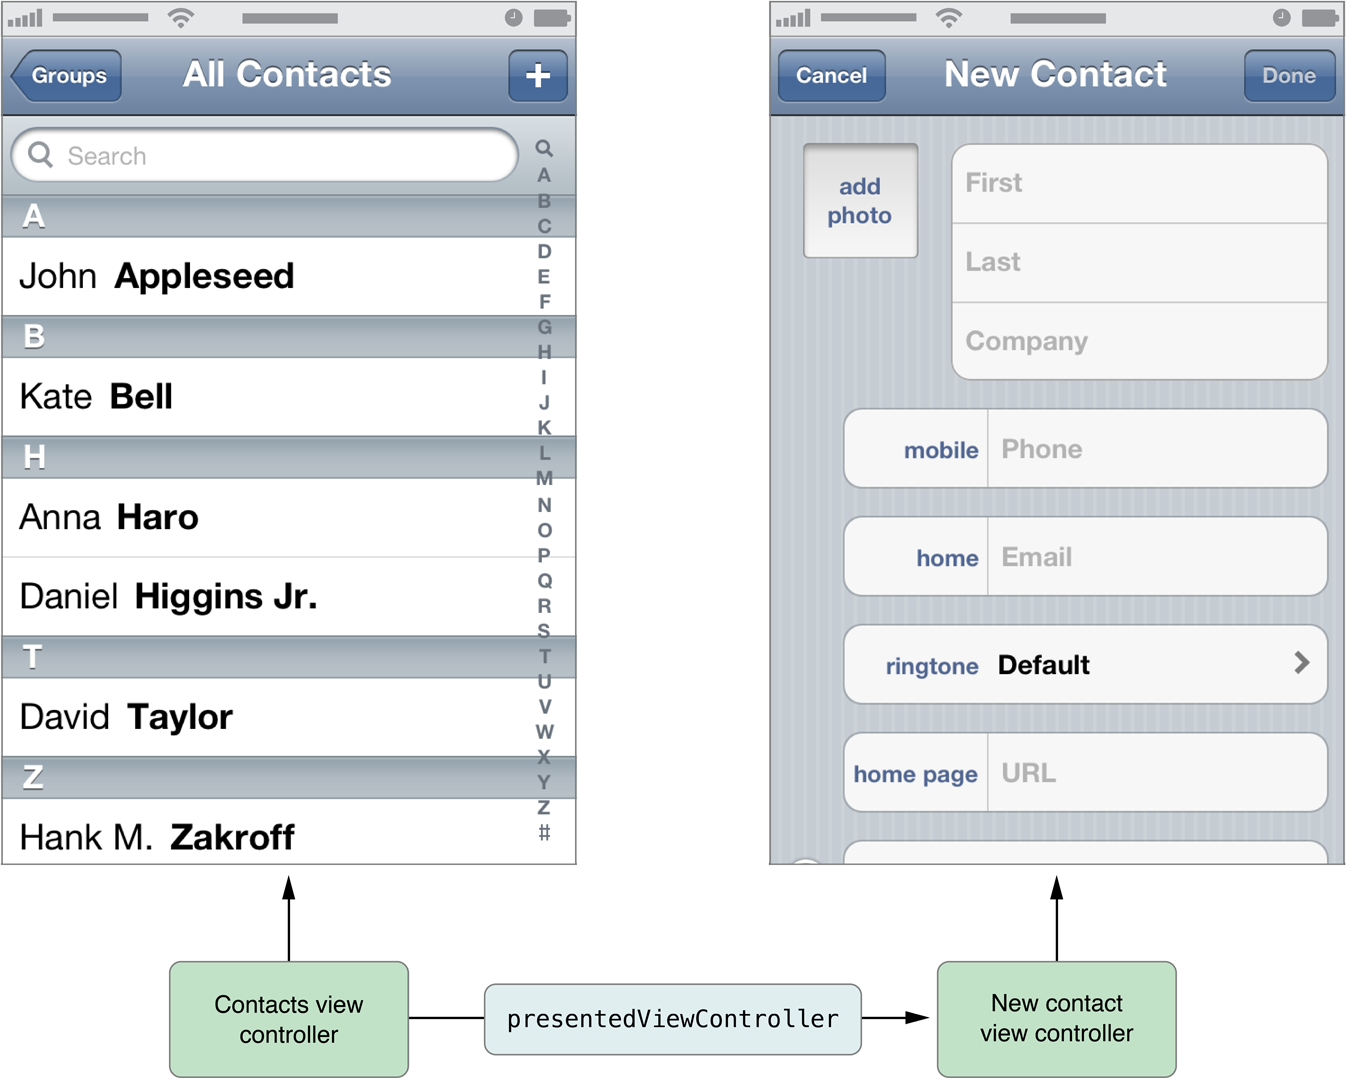
\includegraphics[totalheight=0.4\textheight]{figuras/apple_table_view_controller_contatos.png}
  \caption{Exemplo de tela com lista de contatos que chama tela com lista de atributos}
  \label{fig:a}
\end{figure}

\paragraph{}É interessante que você acompanhe o tutorial junto com a documentação da Apple sobre \texttt{\textbf{UITableViewController}}, e no final busque novos tipos de interação com o usuário e customização da tabela. Não é a toa que essa estrutura é tão explorada nos aplicativos, há uma gama muito grande de possibilidades para seu uso.\\

\paragraph{}Crie um novo projeto da mesma forma que fizemos com o primeiro aplicativo, e coloque "Table" como nome. Agora abra o arquivo \texttt{\textbf{TableViewController.m}} e na declaração da classe adicione \texttt{\textbf{<UITableViewDataSource,UITableViewDelegate>}}.

\begin{listing}
\begin{minted}[linenos=true,frame=lines,framesep=2mm,tabsize=2,numbersep=5pt]{objective-c}
@interface TableViewController : UIViewController <UITableViewDataSource,UITableViewDelegate>
\end{minted}
\end{listing}

\paragraph{}Assim teremos a possibilidade de sobrescrever diversos métodos de \texttt{\textbf{da UITableView}} que já são chamados pela controladora para gerenciar o comportamento e as configurações da tabela.
\paragraph{}Métodos como esse:

\begin{listing}
\begin{minted}[linenos=true,frame=lines,framesep=2mm,tabsize=2,numbersep=5pt]{objective-c}
- (NSInteger)tableView:(UITableView *)tableView numberOfRowsInSection:(NSInteger)section
\end{minted}
\end{listing}

\paragraph{}Que retorna o número de linhas por seção. E esse:

\begin{listing}
\begin{minted}[linenos=true,frame=lines,framesep=2mm,tabsize=2,numbersep=5pt]{objective-c}
- (UITableViewCell *)tableView:(UITableView *)tableView cellForRowAtIndexPath:(NSIndexPath *)indexPath
\end{minted}
\end{listing}

Que é chamado no carregamento de cada célula da tabela e retorna um objeto \texttt{\textbf{UITableViewCell}} que contém as definições dessa celula, como texto, imagem de fundo, ou uma imagem miniatura. O endereço da célula é obtido pelo parâmetro \texttt{\textbf{indexPath}}, que contém dois valores: a seção (\texttt{\textbf{section}}) e a linha (\texttt{\textbf{row}}).
\paragraph{}Vamos carregar os dados dos contatos a partir de uma property list chamada \texttt{\textbf{contatos.plis}} já criada e presente no repositório. Adicione este arquivo no projeto e abra-o para entender como os contatos estão estruturados. A ideia é dividir os contatos pela letra inicial, tornando cada letra existente uma chave primária para a estrutura. Dessa forma podemos montar esses dados em um dicionário e facilitar a busca e a ordenação dos contatos.
\paragraph{}Antes dessa leitura, é preciso criar uma classe modelo para o contato. A classe é simples, vai conter apenas nome, sobrenome, e número. Para isso, basta criar um novo arquivo da mesma que fizemos até agora, herdando simplesment de \texttt{\textbf{NSObject}}. Usaremos o nome \texttt{\textbf{DataContato}}.
\paragraph{}No arquivo \texttt{\textbf{DataContato.h}} colocaremos apenas as 3 propriedades da classe, e um método construtor.

\begin{listing}
\begin{minted}[linenos=true,frame=lines,framesep=2mm,tabsize=2,numbersep=5pt]{objective-c}
@interface DataContato : NSObject

@property (nonatomic, retain) NSString *firstName;
@property (nonatomic, retain) NSString *lastName;
@property (nonatomic, retain) NSString *numero;

- (id)initWithFirstName:(NSString *)aFirstName
               lastName:(NSString *)aLastName
                 numero:(NSString *)aNumero;

@end
\end{minted}
\end{listing}

\paragraph{}E no arquivo \texttt{\textbf{DataContato.m}} colocamos a implementação do construtor.

\begin{listing}
\begin{minted}[linenos=true,frame=lines,framesep=2mm,tabsize=2,numbersep=5pt]{objective-c}
@implementation DataContato

- (id)init
{
    return [self initWithFirstName:@"N/A"
                          lastName:@"N/A"
                            numero:@"N/A"];
}

- (id)initWithFirstName:(NSString *)aFirstName
               lastName:(NSString *)aLastName
                 numero:(NSString *)aNumero;
{    
    self.firstName = aFirstName;
    self.lastName = aLastName;
    self.numero = aNumero;
    
    return self;
}

@end
\end{minted}
\end{listing}

Com o modelo pronto, podemos montar o arquivo \texttt{\textbf{contato.plist}} em um dicionário de uma forma que os dados tenham sentido. É preciso importar a classe em \texttt{\textbf{TableViewController.h}} e criar as propriedades e métodos que utilizaremos para gerenciar a estrutura dos contatos e orderná-los.
\paragraph{}Em um projeto maior, o mais correto seria implementar o gerenciamento e lógica da estrutura de dados em uma classe separada, para manter o código organizado. Mas por enquanto vamos colocar a lógica na \texttt{\textbf{TableViewController}} mesmo para deixar mais simples.

\begin{listing}
\begin{minted}[linenos=true,frame=lines,framesep=2mm,tabsize=2,numbersep=5pt]{objective-c}
#import "DataContato.h"

@interface TableViewController : UIViewController <UITableViewDataSource,UITableViewDelegate>

@property (nonatomic, retain) NSMutableDictionary *dictionary;
@property (nonatomic, retain) NSMutableArray *keysArray;
@property (nonatomic, retain) NSMutableArray *contatoObjArray;

- (void) setDictionaryArray;
- (void) sortObjArray:(NSMutableArray *)arrayObj;

@end
\end{minted}
\end{listing}

A propriedade \texttt{\textbf{dicionary}} vai ser o nosso dicionário, contendo todos os dados do arquivo \texttt{\textbf{contatos.plist}}, desordenados e sem significado. Em \texttt{\textbf{keysArray}} salvaremos um \emph{array} com as primeiras letras dos contatos, assim podemos buscar os dados em \texttt{\textbf{dictionary}} para enfim transformá-los em objetos \texttt{\textbf{DataContato}}, e salvá-los em \texttt{\textbf{ContatoObjArray}}, divididos entre as letras.

\bigskip
\bigskip
\bigskip
\bigskip

Agora vamos para o arquivo de implementação. Esse será nosso método \texttt{\textbf{viewDidLoad}}:

\begin{listing}
\begin{minted}[linenos=true,frame=lines,framesep=2mm,tabsize=2,numbersep=5pt]{objective-c}
- (void)viewDidLoad
{
    [super viewDidLoad];
    
    self.navigationItem.title = @"Contatos";
    
    NSString *filePath = [[NSBundle mainBundle]
    					pathForResource:@"contatos"
    					ofType:@"plist"];
    
    self.dictionary = [[NSMutableDictionary alloc]
    				   initWithContentsOfFile:filePath];
    
    [self setDictionaryArray];
}
\end{minted}
\end{listing}

Nesse código, primeiro damos à tela o título Contatos, e então vamos montar o endereço do arquivo \texttt{\textbf{contatos.plist}} na variável \texttt{\textbf{filePath}}. Podemos então inicializar a propriedade \texttt{\textbf{dictionary}} com o conteúdo desse endereço. Por último chamamos o método \texttt{\textbf{setDictionaryArray}}, que será onde montaremos a estrutura dos contatos utilizando as chaves primárias e a classe \texttt{\textbf{DataContato}}.
\paragraph{}Agora vamos montar o método \texttt{\textbf{setDictionaryArray}} por partes. Vamos primeiro separar as chaves primárias e ordená-las utilizando um objeto \texttt{\textbf{NSSortDescriptor}}:

\begin{listing}
\begin{minted}[linenos=true,frame=lines,framesep=2mm,tabsize=2,numbersep=5pt]{objective-c}
NSMutableArray *tmpKey, *tmpContato;
    NSString *firstNameAux, *lastNameAux, *numeroAux;
    
    NSSortDescriptor *sort = [NSSortDescriptor sortDescriptorWithKey:nil ascending:YES];
    
    self.keysArray = [[NSMutableArray alloc] initWithArray:[self.dictionary allKeys]];
    [self.keysArray sortUsingDescriptors:[NSArray arrayWithObject:sort]];
    
    int countKeys = [self.keysArray count];

    NSMutableArray *arrayObj = [[NSMutableArray alloc] init];
\end{minted}
\end{listing}

\paragraph{}Este código mostra um modo mais simples de ordenação de um \texttt{\textbf{NSArray}} com um \texttt{\textbf{NSSortDescriptor}}. Criamos o objeto \texttt{\textbf{sort}} e setamos que a ordenação vai ser ascendente, então salvamos em \texttt{\textbf{keysArray}} todas as chaves de \texttt{\textbf{dictionary}} utilizando o método \texttt{\textbf{allKeys}} de \texttt{\textbf{NSDictionary}}. Por fim fazemos a ordenação de \texttt{\textbf{keysArray}} com o método \texttt{\textbf{sortUsingDescriptors}}, onde mandamos como parâmetro um \texttt{\textbf{NSArray}} criado com o \texttt{\textbf{sort}}.

\paragraph{}Sempre que vamos fazer uma ordenação de um \texttt{\textbf{NSArray}}, devemos criar um ou mais objeto \texttt{\textbf{NSSortDescriptor}} (podemos ter mais de um fato de ordenação, como veremos mais a frente) e criamos um novo\texttt{\textbf{NSArray}} contendo esses objetos. Com o \texttt{\textbf{NSArray}} a ser ordenado e o \texttt{\textbf{NSArray}} de ordenação, já temos tudo que é preciso para o método resolver o problema.

\paragraph{}Agora continuamos com o método, e faremos um laço para separar os contatos de cada letra, utilizando métodos do \texttt{\textbf{NSDictionary}} para obter o conteúdo de cada chave. E dentro mais um laço para separar os dados de cada contato. Assim, podemos criar novas instâncias de \texttt{\textbf{DataContato}} com os dados obtidos da estrutura de \texttt{\textbf{dictionary}}.

\begin{listing}
\begin{minted}[linenos=true,frame=lines,framesep=2mm,tabsize=2,numbersep=5pt]{objective-c}
for (int i=0; i<countKeys; i++)
    {
	 tmpKey = [[NSMutableArray alloc] init];
        tmpKey = [NSMutableArray arrayWithArray:[self.dictionary objectForKey:[self.keysArray objectAtIndex:i]]];
        
        NSMutableArray *arrayObjAux = [[NSMutableArray alloc] init];
        
        for (int j=0; j<[tmpKey count]; j++)
        {
            tmpContato = [[NSMutableArray alloc] initWithArray:[tmpKey objectAtIndex:j]];

            firstNameAux = [[NSString alloc] initWithString:[tmpContato objectAtIndex:0]];
            lastNameAux = [[NSString alloc] initWithString:[tmpContato objectAtIndex:1]];
            numeroAux = [[NSString alloc] initWithString:[tmpContato objectAtIndex:2]];
            
            DataContato *a = [[DataContato alloc] initWithFirstName:firstNameAux
                                                           lastName:lastNameAux
                                                             numero:numeroAux];
            
            [arrayObjAux addObject:a];            
        }
        
        [arrayObj addObject:arrayObjAux];
    }
\end{minted}
\end{listing}

Finalizando o método, fazemos a chamada do método que vai ordenar o \emph{array} de objetos \texttt{\textbf{DataContato}} produzido, ordenando internamente os contatos de cada chave primária de acordo com nome e sobrenome.

\begin{listing}
\begin{minted}[linenos=true,frame=lines,framesep=2mm,tabsize=2,numbersep=5pt]{objective-c}
[self sortObjArray:arrayObj];
\end{minted}
\end{listing}

Neste método \texttt{\textbf{sortObjArray}}, faremos um uso mais específico do \texttt{\textbf{NSSortDescriptor}}, que nos permite alguns truques de ordenação. Vamos ordernar primeiro por nome e depois por sobrenome, e realocar o contato inteiro e não cada atributo separado. Assim como fizemos no método anterior, vamos definir nossas prioridades de ordenação em um \texttt{\textbf{NSArray}}, e utilizar um método parecido de \texttt{\textbf{NSArray}} para ordernar automaticamente o \emph{array} de contatos de cada letra.\\
\paragraph{}Vamos criar o método \texttt{\textbf{sortObjArray}} por partes. Primeiro criamos os dois arquivos de ordenação, um pra nome e outro pra sobrenome.

\bigskip
\bigskip

\begin{listing}
\begin{minted}[linenos=true,frame=lines,framesep=2mm,tabsize=2,numbersep=5pt]{objective-c}
self.contatoObjArray = [[NSMutableArray alloc] init];
    
    // ordenar Nomes
    NSString *LASTNAME = @"lastName";
    NSString *FIRSTNAME = @"firstName";
    
    // Descriptor do sobrenome
    NSSortDescriptor *lastDescriptor =
    [[NSSortDescriptor alloc]
      initWithKey:LASTNAME
      ascending:YES
      selector:@selector(localizedCaseInsensitiveCompare:)];
    
    // Descriptor do nome
    NSSortDescriptor *firstDescriptor =
    [[NSSortDescriptor alloc]
      initWithKey:FIRSTNAME
      ascending:YES
      selector:@selector(localizedCaseInsensitiveCompare:)];
\end{minted}
\end{listing}

Cada \emph{descriptor} vai ser responsável pela ordenação de um atributo do objeto \texttt{\textbf{DataContato}}. Definimos qual vai ser o atributo nos parâmetros, e utilizamos um \emph{selector} que não vai diferenciar letras maiúsculas e minúsculas.

\paragraph{}O \texttt{\textbf{NSSortDescriptor}} é uma biblioteca muito poderosa para ordenação, que vale a pena ser um pouco mais estudada.
\paragraph{}Finalizamos o método criando um \emph{array} com a nossa prioridade de ordenação, e criamos um laço que vai pegar o \emph{array} de cada letra e ordenar com o método \texttt{\textbf{sortedArrayUsingDescriptors}} que recebe o nosso \emph{array} com a prioridade.

\begin{listing}
\begin{minted}[linenos=true,frame=lines,framesep=2mm,tabsize=2,numbersep=5pt]{objective-c}
NSArray * descriptors =
    [NSArray arrayWithObjects:firstDescriptor, lastDescriptor, nil];
      
    for(NSMutableArray* array in arrayObj)
        [self.contatoObjArray addObject:[array sortedArrayUsingDescriptors:descriptors]];
\end{minted}
\end{listing}

\bigskip
\bigskip

Com a nossa estrutura de dados pronta, podemos enfim criar um objeto \texttt{\textbf{UITableView}} em \texttt{\textbf{UITableViewController}} para começarmos a lidar com os dados na tela.
\paragraph{}Adicione a tabela pelo \emph{Interface Builder} da mesma forma que já fizemos. Apague tudo que já existir na tela, selecione \texttt{\textbf{Table View}} entre os objetos e arraste para a tela. Então selecione a tabela adicionada e arraste-a com o Ctrl apertado para o código do \emph{header} ao lado para criar um \emph{outlet}. Crie-o com o nome \texttt{\textbf{table}}. Além disso, é preciso fazer a ligação com o \emph{File's Owner} para indicar que as alterações feitas no código da \texttt{\textbf{UITableViewController}} terão efeito na tabela. Para isso, basta selecionar a tabela e arrastar com o Ctrl apertado até o quadrado amarelo no lado esquerdo. Selecione \texttt{\textbf{dataSource}}, e faça mais uma vez para selecionar \texttt{\textbf{delegate}}.

\paragraph{}Agora temos nossa tabela pronta para uso, devemos então customizá-la sobrescrevendo seus métodos. Para definir características de exibição da tabela, utilizaremos por enquanto 5 métodos básicos: número de seções (total de letras), número de linhas por seção (total de contatos por letra), título de cada seção (cada letra), o índice de seções na lateral (o \emph{array} de letras), e o que será exibido em cada célula (cada contato). Vamos passar devagar por cada um dos métodos.

\paragraph{}Os métodos de contagem são bem simples, retornando simplesmente o total de cada \texttt{\textbf{NSArray}}.

\begin{listing}
\begin{minted}[linenos=true,frame=lines,framesep=2mm,tabsize=2,numbersep=5pt]{objective-c}
- (NSInteger)numberOfSectionsInTableView:(UITableView *)tableView
{
    return [self.keysArray count];
}

- (NSInteger)tableView:(UITableView *)tableView
 numberOfRowsInSection:(NSInteger)section
{
    return [[self.dictionary objectForKey:[self.keysArray objectAtIndex:section]] count];
}
\end{minted}
\end{listing}

\bigskip
\bigskip

No primeiro método, retornamos o total de elementos de \texttt{\textbf{keysArray}}. O segundo método tem a mesma ideia, mas é necessário utilizar o parâmetro \texttt{\textbf{section}} para buscar o total de contatos de acordo com a letra, já que esse valor é variável.
\paragraph{}O método \texttt{\textbf{objectForKey}} de \texttt{\textbf{NSDictionary}} retorna o conteúdo de uma dada chave do dicionário, e o método \texttt{\textbf{objectAtIndex}} de \texttt{\textbf{NSArray}} retorna o conteúdo de uma dada posição do \emph{array}.

\begin{listing}
\begin{minted}[linenos=true,frame=lines,framesep=2mm,tabsize=2,numbersep=5pt]{objective-c}
- (NSString *)tableView:(UITableView *)tableView titleForHeaderInSection:(NSInteger)section
{
    return [self.keysArray objectAtIndex:section];
}

- (NSArray *)sectionIndexTitlesForTableView:(UITableView *)tableView
{    
    return [self.keysArray];
}
\end{minted}
\end{listing}

\bigskip
\bigskip

Seguindo a mesma ideia dos métodos anteriores, neste primeiro método retornamos a letra contida na posição correspondente ao valor de \texttt{\textbf{section}} em \texttt{\textbf{keysArray}}. No segundo método, definimos um índice para a lista de contatos retornando o próprio \texttt{\textbf{keysArray}} que contém todas as letras ordenadas.
\paragraph{}Por enquanto já temos definido a organização das seções e linhas da tabela, faltando apenas determinar o que cada célula vai exibir. Vamos definir a construção e conteúdo das celulas com seguinte método:

\begin{listing}
\begin{minted}[linenos=true,frame=lines,framesep=2mm,tabsize=2,numbersep=5pt]{objective-c}
- (UITableViewCell *) tableView:(UITableView *)tableView cellForRowAtIndexPath:(NSIndexPath *)indexPath {
    
    static NSString *MyIdentifier = @"MyIdentifier";
    
    UITableViewCell *cell = [tableView dequeueReusableCellWithIdentifier:MyIdentifier];
    if(cell == nil) {
        cell = [[UITableViewCell alloc] initWithStyle:UITableViewCellStyleDefault
                                      reuseIdentifier:MyIdentifier];
    }

    DataContato *a = [[self.contatoObjArray objectAtIndex:indexPath.section] objectAtIndex:indexPath.row];

    NSString *texto = a.firstName;
    cell.textLabel.text = texto;
        
    UIImage *cellImage = [UIImage imageNamed:@"apple.png"];
        
    cell.imageView.image = cellImage;
    
    return cell;
}
\end{minted}
\end{listing}

\bigskip
\bigskip

A primeira parte do método é um código padrão que serve para reutilizar células, e criar apenas o número de células exibidas na tela, atualizando o conteúdo de acordo com a rolagem feita pelo usuário. O processo de criação das células é custoso, sendo desnescessário criar uma célula para cada linha que será exibida, bastando apenas criar um número fixo e reutilizar. Não é preciso entender exatamente o que esse trecho faz, apenas copie-o.
\paragraph{}Na segunda parte temos a criação do conteúdo de fato, utilizando o parâmetro \texttt{\textbf{indexPath}}. Como dito anteriormente, o \texttt{\textbf{indexPath}} possui os atributos \texttt{\textbf{section}}, com o número da seção, e \texttt{\textbf{row}}, com o número da linha. Ele funciona como o posicionamento de uma matriz, e graças a ela podemos definir conteúdo variável nas células.
\paragraph{}Este método é chamado na criação de cada célula da tabela, e retorna o objeto \texttt{\textbf{cell}} do tipo \texttt{\textbf{UITableViewCell}}, que nada mais é que o pacote de conteúdo e características de uma célula, com diversos atributos que definem a célula.
\paragraph{}Vamos então instanciar um objeto \texttt{\textbf{DataContato}} de acordo com os valores de \texttt{\textbf{section}} e \texttt{\textbf{row}}, que darão a posição do objeto em \texttt{\textbf{contatoObjArray}}. Então salvamos apenas a \emph{string} do primeiro nome em \texttt{\textbf{cell.textLabel.text}}, onde \texttt{\textbf{textLabel}} é um atributo do tipo \texttt{\textbf{UILabel}} que determina o texto que é exibido na célula e suas características.
\paragraph{}Além disso, vamos determinar uma imagem a ser exibida na célula. No caso utilizei uma imagem bem simples, contida no repositório, com o logo da Apple, mas você pode colocar outra imagem em .png se quiser, bastando colocar o nome da imagem no parâmetro correspondente. Essa imagem será então salva em \texttt{\textbf{cell.imageView.image}}. Note que, se cada contato tiver uma imagem customizada, é possível determinar um \texttt{\textbf{NSArray}} com o nome da imagem correspondente a cada contato, e utilizar o \texttt{\textbf{indexPath}} da mesma forma que o utilizamos para determinar o texto da célula.

\bigskip
\bigskip

\paragraph{}Pronto, já temos a exibição dos contatos funcionando. O próximo passo é criar uma tela de exibição dos detalhes do contato, que também usará uma \texttt{\textbf{UITableView}} e que será chamada quando a célula de um contato for clicado.
\paragraph{}Crie uma nova tela herdando de \texttt{\textbf{UIViewController}} chamada \texttt{\textbf{Detail}}. Assim como fizemos na \texttt{\textbf{TableViewController}}, adicione uma \texttt{\textbf{UITableView}} na tela (que chamei de \texttt{\textbf{tableDetail}}), crie o \texttt{\textbf{outlet}}, faça as ligações com o \texttt{\textbf{File's Owner}}, e por fim mude a declaração da classe no arquivo header \texttt{\textbf{Detail.h}}.

\begin{listing}
\begin{minted}[linenos=true,frame=lines,framesep=2mm,tabsize=2,numbersep=5pt]{objective-c}
@interface Detail : UIViewController <UITableViewDataSource,UITableViewDelegate>
\end{minted}
\end{listing}

Por último, faremos uma alteração no \emph{layout} da tabela. No \emph{Interface Builder}, abra o menu \emph{Utilities} à direita, selecione a tabela e vá em \emph{Attributes Inspector}, e lá mude o atributo \emph{Style} de \emph{Plain} para \emph{Grouped}. Como teremos uma lista pequena com apenas uma \texttt{\textbf{section}}, esse layout parece mais adequado.
\paragraph{}Além da tabela, vamos criar mais uma única propriedade que será uma instância de \texttt{\textbf{DataContato}}, que chamaremos simplesmente de \texttt{\textbf{contato}}. A ideia é que quando uma célula de \texttt{\textbf{TableViewController}} for tocada, a tela \texttt{\textbf{Detail}} será chamada e o contato correspondente à celula será salvo em \texttt{\textbf{contato}} para que todos seus atributos sejam exbidos na tabela. A classe em \texttt{\textbf{Detail.h}} deve ficar assim:

\begin{listing}
\begin{minted}[linenos=true,frame=lines,framesep=2mm,tabsize=2,numbersep=5pt]{objective-c}
@interface Detail : UIViewController <UITableViewDataSource,UITableViewDelegate>

@property (weak, nonatomic) IBOutlet UITableView *tableDetail;

@property (nonatomic, retain) DataContato *contato;

@end
\end{minted}
\end{listing}

Partiremos agora para a implementação. O código nessa tela é bem mais simples que em \texttt{\textbf{TableViewController}}, já que o tamanho da tabela é fixo e o conteúdo a ser exibido virá sempre de \texttt{\textbf{contato}}.

\texttt{\textbf{}}

- TELA COM DETALHES DO CONTATO\\
- CLIQUE NA TABELA\\
- PERMITIR LIGAÇÃO\\
- BUSCA\\

\bigskip
\bigskip


%%%%%%%%%%%%%%%%%%%%%%%%%%%%%%%%%%%%%%%%%%%%%%%%%%%%%%%%%%%%%%%%%%%%%%%%%%%%%%%%

\singlespace
\selectlanguage{brazil}
\cleardoublepage
\thispagestyle{empty}
\phantomsection
\addcontentsline{toc}{chapter}{Referências Bibliográficas}
\bibliography{../comum/biblio}
\bibliographystyle{apalike}
\doublespace


\appendix
\addtocontents{toc}{\protect\setcounter{tocdepth}{0}} % as seções do apêndice não aparecem do sumário com este comando...
%%%%%%%%%%%%%%%%%%%%%%%%%%%%%%%%%%%%%%%%%%%%%%%%%%%%%%%%%%%%%%%%%%%%%%%%%%%%%%%%
\ape{apen}{Especificação blá, blá, blá}

Isto é um apêndice...

%%%%%%%%%%%%%%%%%%%%%%%%%%%%%%%%%%%%%%%%%%%%%%%%%%%%%%%%%%%%%%%%%%%%%%%%%%%%%%%%
\addtocontents{toc}{\protect\setcounter{tocdepth}{1}}

\end{document}
